\documentclass[a4paper]{book}
\usepackage{a4wide}
\usepackage{makeidx}
\usepackage{graphicx}
\usepackage{multicol}
\usepackage{float}
\usepackage{listings}
\usepackage{color}
\usepackage{textcomp}
\usepackage{alltt}
\usepackage{times}
\usepackage{ifpdf}
\ifpdf
\usepackage[pdftex,
            pagebackref=true,
            colorlinks=true,
            linkcolor=blue,
            unicode
           ]{hyperref}
\else
\usepackage[ps2pdf,
            pagebackref=true,
            colorlinks=true,
            linkcolor=blue,
            unicode
           ]{hyperref}
\usepackage{pspicture}
\fi
\usepackage[utf8]{inputenc}
\usepackage{doxygen}
\lstset{language=C++,inputencoding=utf8,basicstyle=\footnotesize,breaklines=true,breakatwhitespace=true,tabsize=8,numbers=left }
\makeindex
\setcounter{tocdepth}{3}
\renewcommand{\footrulewidth}{0.4pt}
\begin{document}
\hypersetup{pageanchor=false}
\begin{titlepage}
\vspace*{7cm}
\begin{center}
{\Large TR3D }\\
\vspace*{1cm}
{\large Generated by Doxygen 1.7.0}\\
\vspace*{0.5cm}
{\small Fri Jun 24 2011 11:45:59}\\
\end{center}
\end{titlepage}
\clearemptydoublepage
\pagenumbering{roman}
\tableofcontents
\clearemptydoublepage
\pagenumbering{arabic}
\hypersetup{pageanchor=true}
\chapter{Class Index}
\section{Class Hierarchy}
This inheritance list is sorted roughly, but not completely, alphabetically:\begin{DoxyCompactList}
\item \contentsline{section}{AnimationClip}{\pageref{struct_animation_clip}}{}
\item \contentsline{section}{CollisionHandler}{\pageref{class_collision_handler}}{}
\item \contentsline{section}{CollisionHit}{\pageref{struct_collision_hit}}{}
\item \contentsline{section}{GameObjectFactory}{\pageref{class_game_object_factory}}{}
\item \contentsline{section}{KeyFrame}{\pageref{struct_key_frame}}{}
\item \contentsline{section}{LightFactory}{\pageref{class_light_factory}}{}
\item \contentsline{section}{LightManager}{\pageref{class_light_manager}}{}
\item \contentsline{section}{Object}{\pageref{class_object}}{}
\begin{DoxyCompactList}
\item \contentsline{section}{Component}{\pageref{class_component}}{}
\begin{DoxyCompactList}
\item \contentsline{section}{Animation}{\pageref{class_animation}}{}
\item \contentsline{section}{Behaviour}{\pageref{class_behaviour}}{}
\begin{DoxyCompactList}
\item \contentsline{section}{DebugCamera}{\pageref{class_debug_camera}}{}
\end{DoxyCompactList}
\item \contentsline{section}{Camera}{\pageref{class_camera}}{}
\item \contentsline{section}{Collider}{\pageref{class_collider}}{}
\begin{DoxyCompactList}
\item \contentsline{section}{BoxCollider}{\pageref{class_box_collider}}{}
\item \contentsline{section}{PlaneCollider}{\pageref{class_plane_collider}}{}
\item \contentsline{section}{SphereCollider}{\pageref{class_sphere_collider}}{}
\end{DoxyCompactList}
\item \contentsline{section}{GLSLShader}{\pageref{class_g_l_s_l_shader}}{}
\item \contentsline{section}{Light}{\pageref{class_light}}{}
\item \contentsline{section}{Material}{\pageref{class_material}}{}
\item \contentsline{section}{Renderable}{\pageref{class_renderable}}{}
\begin{DoxyCompactList}
\item \contentsline{section}{MeshRenderer}{\pageref{class_mesh_renderer}}{}
\begin{DoxyCompactList}
\item \contentsline{section}{CubeMeshRenderer}{\pageref{class_cube_mesh_renderer}}{}
\item \contentsline{section}{PlaneMeshRenderer}{\pageref{class_plane_mesh_renderer}}{}
\item \contentsline{section}{SphereMeshRenderer}{\pageref{class_sphere_mesh_renderer}}{}
\end{DoxyCompactList}
\item \contentsline{section}{ParticleSystem}{\pageref{class_particle_system}}{}
\item \contentsline{section}{Terrain}{\pageref{class_terrain}}{}
\end{DoxyCompactList}
\item \contentsline{section}{Texture}{\pageref{class_texture}}{}
\end{DoxyCompactList}
\item \contentsline{section}{GameObject}{\pageref{class_game_object}}{}
\item \contentsline{section}{TR3D::TriMesh}{\pageref{class_t_r3_d_1_1_tri_mesh}}{}
\item \contentsline{section}{Transform}{\pageref{class_transform}}{}
\end{DoxyCompactList}
\item \contentsline{section}{Pointer$<$ T $>$}{\pageref{class_pointer}}{}
\item \contentsline{section}{Ray}{\pageref{struct_ray}}{}
\item \contentsline{section}{RayCastHit}{\pageref{struct_ray_cast_hit}}{}
\item \contentsline{section}{Ressource}{\pageref{class_ressource}}{}
\begin{DoxyCompactList}
\item \contentsline{section}{Texture}{\pageref{class_texture}}{}
\item \contentsline{section}{TR3D::TriMesh}{\pageref{class_t_r3_d_1_1_tri_mesh}}{}
\end{DoxyCompactList}
\item \contentsline{section}{RessourceManager}{\pageref{class_ressource_manager}}{}
\item \contentsline{section}{RTTI}{\pageref{class_r_t_t_i}}{}
\item \contentsline{section}{Scene}{\pageref{class_scene}}{}
\item \contentsline{section}{Screen}{\pageref{class_screen}}{}
\item \contentsline{section}{TrackBallCamera}{\pageref{class_track_ball_camera}}{}
\item \contentsline{section}{TREngine}{\pageref{class_t_r_engine}}{}
\item \contentsline{section}{Vertex}{\pageref{struct_vertex}}{}
\end{DoxyCompactList}

\chapter{Class Index}
\section{Class List}
Here are the classes, structs, unions and interfaces with brief descriptions:\begin{DoxyCompactList}
\item\contentsline{section}{\hyperlink{class_animation}{Animation} }{\pageref{class_animation}}{}
\item\contentsline{section}{\hyperlink{struct_animation_clip}{AnimationClip} }{\pageref{struct_animation_clip}}{}
\item\contentsline{section}{\hyperlink{class_behaviour}{Behaviour} }{\pageref{class_behaviour}}{}
\item\contentsline{section}{\hyperlink{class_box_collider}{BoxCollider} }{\pageref{class_box_collider}}{}
\item\contentsline{section}{\hyperlink{class_camera}{Camera} }{\pageref{class_camera}}{}
\item\contentsline{section}{\hyperlink{class_collider}{Collider} }{\pageref{class_collider}}{}
\item\contentsline{section}{\hyperlink{class_collision_handler}{CollisionHandler} }{\pageref{class_collision_handler}}{}
\item\contentsline{section}{\hyperlink{struct_collision_hit}{CollisionHit} }{\pageref{struct_collision_hit}}{}
\item\contentsline{section}{\hyperlink{class_component}{Component} }{\pageref{class_component}}{}
\item\contentsline{section}{\hyperlink{class_cube_mesh_renderer}{CubeMeshRenderer} }{\pageref{class_cube_mesh_renderer}}{}
\item\contentsline{section}{\hyperlink{class_debug_camera}{DebugCamera} }{\pageref{class_debug_camera}}{}
\item\contentsline{section}{\hyperlink{class_game_object}{GameObject} }{\pageref{class_game_object}}{}
\item\contentsline{section}{\hyperlink{class_game_object_factory}{GameObjectFactory} }{\pageref{class_game_object_factory}}{}
\item\contentsline{section}{\hyperlink{class_g_l_s_l_shader}{GLSLShader} }{\pageref{class_g_l_s_l_shader}}{}
\item\contentsline{section}{\hyperlink{struct_key_frame}{KeyFrame} }{\pageref{struct_key_frame}}{}
\item\contentsline{section}{\hyperlink{class_light}{Light} }{\pageref{class_light}}{}
\item\contentsline{section}{\hyperlink{class_light_factory}{LightFactory} }{\pageref{class_light_factory}}{}
\item\contentsline{section}{\hyperlink{class_light_manager}{LightManager} }{\pageref{class_light_manager}}{}
\item\contentsline{section}{\hyperlink{class_material}{Material} }{\pageref{class_material}}{}
\item\contentsline{section}{\hyperlink{class_mesh_renderer}{MeshRenderer} }{\pageref{class_mesh_renderer}}{}
\item\contentsline{section}{\hyperlink{class_object}{Object} }{\pageref{class_object}}{}
\item\contentsline{section}{\hyperlink{class_particle_system}{ParticleSystem} }{\pageref{class_particle_system}}{}
\item\contentsline{section}{\hyperlink{class_plane_collider}{PlaneCollider} }{\pageref{class_plane_collider}}{}
\item\contentsline{section}{\hyperlink{class_plane_mesh_renderer}{PlaneMeshRenderer} }{\pageref{class_plane_mesh_renderer}}{}
\item\contentsline{section}{\hyperlink{class_pointer}{Pointer$<$ T $>$} }{\pageref{class_pointer}}{}
\item\contentsline{section}{\hyperlink{struct_ray}{Ray} }{\pageref{struct_ray}}{}
\item\contentsline{section}{\hyperlink{struct_ray_cast_hit}{RayCastHit} }{\pageref{struct_ray_cast_hit}}{}
\item\contentsline{section}{\hyperlink{class_renderable}{Renderable} }{\pageref{class_renderable}}{}
\item\contentsline{section}{\hyperlink{class_ressource}{Ressource} }{\pageref{class_ressource}}{}
\item\contentsline{section}{\hyperlink{class_ressource_manager}{RessourceManager} }{\pageref{class_ressource_manager}}{}
\item\contentsline{section}{\hyperlink{class_r_t_t_i}{RTTI} }{\pageref{class_r_t_t_i}}{}
\item\contentsline{section}{\hyperlink{class_scene}{Scene} }{\pageref{class_scene}}{}
\item\contentsline{section}{\hyperlink{class_screen}{Screen} }{\pageref{class_screen}}{}
\item\contentsline{section}{\hyperlink{class_sphere_collider}{SphereCollider} }{\pageref{class_sphere_collider}}{}
\item\contentsline{section}{\hyperlink{class_sphere_mesh_renderer}{SphereMeshRenderer} }{\pageref{class_sphere_mesh_renderer}}{}
\item\contentsline{section}{\hyperlink{class_terrain}{Terrain} }{\pageref{class_terrain}}{}
\item\contentsline{section}{\hyperlink{class_texture}{Texture} }{\pageref{class_texture}}{}
\item\contentsline{section}{\hyperlink{class_track_ball_camera}{TrackBallCamera} }{\pageref{class_track_ball_camera}}{}
\item\contentsline{section}{\hyperlink{class_transform}{Transform} }{\pageref{class_transform}}{}
\item\contentsline{section}{\hyperlink{class_t_r_engine}{TREngine} }{\pageref{class_t_r_engine}}{}
\item\contentsline{section}{\hyperlink{class_t_r3_d_1_1_tri_mesh}{TR3D::TriMesh} }{\pageref{class_t_r3_d_1_1_tri_mesh}}{}
\item\contentsline{section}{\hyperlink{struct_vertex}{Vertex} }{\pageref{struct_vertex}}{}
\end{DoxyCompactList}

\chapter{Class Documentation}
\input{class_animation}
\input{struct_animation_clip}
\input{class_behaviour}
\input{class_box_collider}
\input{class_camera}
\input{class_collider}
\input{class_collision_handler}
\input{struct_collision_hit}
\hypertarget{class_component}{
\section{Component Class Reference}
\label{class_component}\index{Component@{Component}}
}
Inheritance diagram for Component:\begin{figure}[H]
\begin{center}
\leavevmode
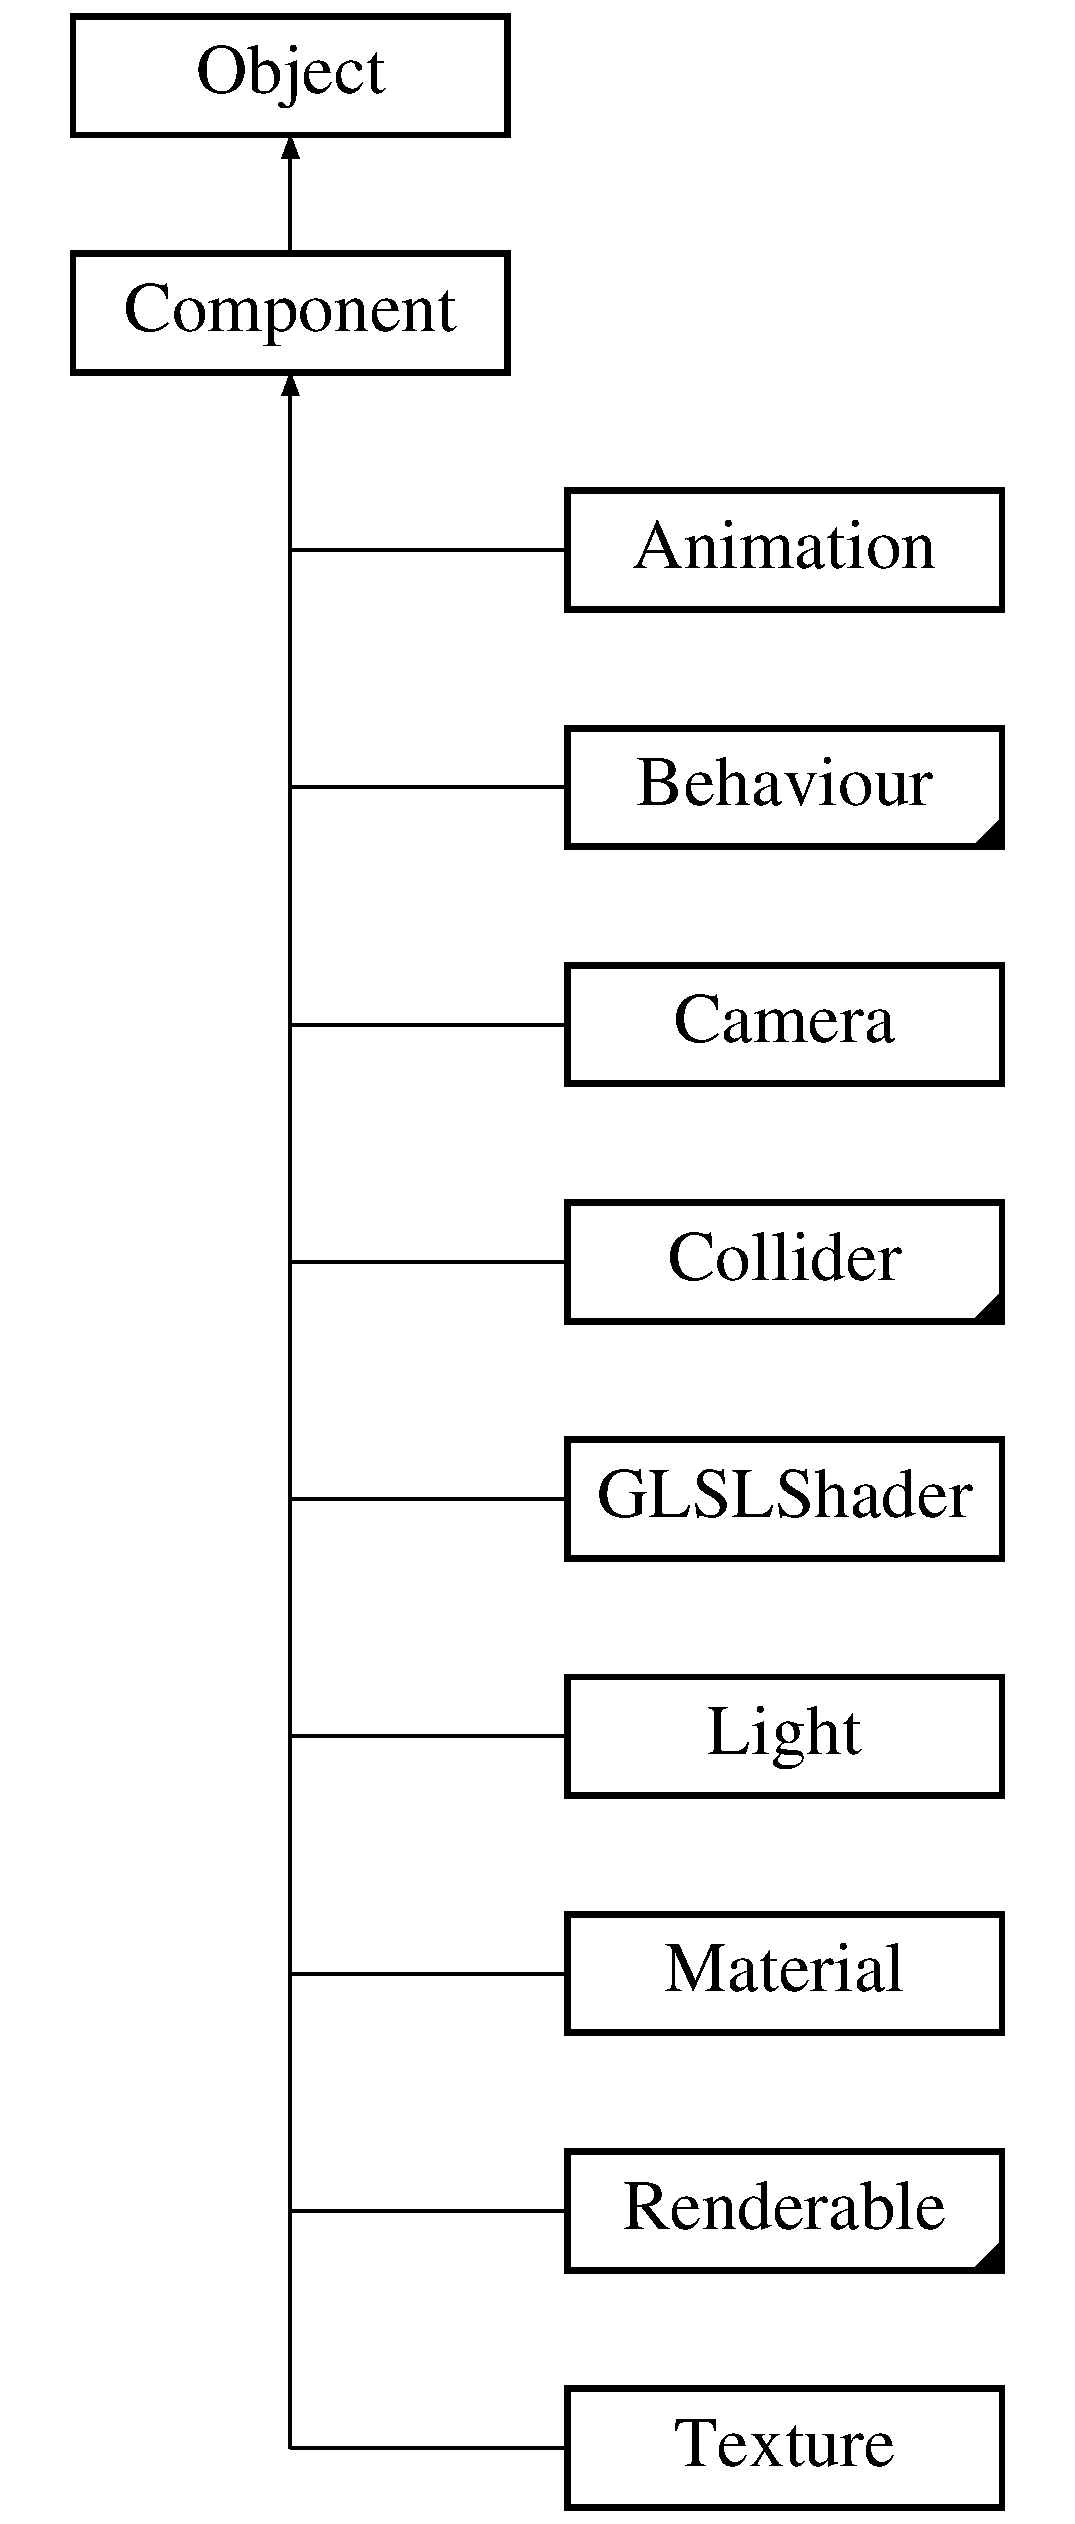
\includegraphics[height=11.000000cm]{class_component}
\end{center}
\end{figure}
\subsection*{Public Member Functions}
\begin{DoxyCompactItemize}
\item 
\hypertarget{class_component_aabc486387d1bbf40f98073e45e6e07b6}{
virtual const \hyperlink{class_r_t_t_i}{RTTI} \& {\bfseries getType} () const }
\label{class_component_aabc486387d1bbf40f98073e45e6e07b6}

\item 
\hypertarget{class_component_abed36db99f1ee0ba84a5fb8485e17428}{
\hyperlink{class_game_object}{GameObject} $\ast$ {\bfseries getGameObject} ()}
\label{class_component_abed36db99f1ee0ba84a5fb8485e17428}

\item 
\hypertarget{class_component_adde518ad6b8f7c51e664fc5a03123f37}{
\hyperlink{class_game_object}{GameObject} const $\ast$const {\bfseries getGameObject} () const }
\label{class_component_adde518ad6b8f7c51e664fc5a03123f37}

\item 
\hypertarget{class_component_a79a940a4c0e948e220c01737efa318de}{
void {\bfseries setGameObject} (\hyperlink{class_game_object}{GameObject} $\ast$obj)}
\label{class_component_a79a940a4c0e948e220c01737efa318de}

\item 
\hypertarget{class_component_ae37c972b61785a3f00604300eb1bcef5}{
virtual Vec3f {\bfseries getWorldPosition} () const }
\label{class_component_ae37c972b61785a3f00604300eb1bcef5}

\item 
\hypertarget{class_component_a68cb3bbdba66799f5a0f4b9b4063fc25}{
virtual Vec3f {\bfseries getPosition} () const }
\label{class_component_a68cb3bbdba66799f5a0f4b9b4063fc25}

\end{DoxyCompactItemize}
\subsection*{Static Public Attributes}
\begin{DoxyCompactItemize}
\item 
\hypertarget{class_component_ac06bcbdc3e5e24713d90276a7df3c6f7}{
static const \hyperlink{class_r_t_t_i}{RTTI} {\bfseries TYPE}}
\label{class_component_ac06bcbdc3e5e24713d90276a7df3c6f7}

\end{DoxyCompactItemize}
\subsection*{Protected Attributes}
\begin{DoxyCompactItemize}
\item 
\hypertarget{class_component_af4a2157b3d021916719085f26f1548b0}{
\hyperlink{class_game_object}{GameObject} $\ast$ {\bfseries gameObject}}
\label{class_component_af4a2157b3d021916719085f26f1548b0}

\item 
\hypertarget{class_component_afa65bb278f1e9256d34d6ea008e654ab}{
bool {\bfseries enabled}}
\label{class_component_afa65bb278f1e9256d34d6ea008e654ab}

\end{DoxyCompactItemize}
\subsection*{Friends}
\begin{DoxyCompactItemize}
\item 
\hypertarget{class_component_ac98d07dd8f7b70e16ccb9a01abf56b9c}{
class {\bfseries boost::serialization::access}}
\label{class_component_ac98d07dd8f7b70e16ccb9a01abf56b9c}

\end{DoxyCompactItemize}


The documentation for this class was generated from the following files:\begin{DoxyCompactItemize}
\item 
Component.h\item 
Component.cpp\end{DoxyCompactItemize}

\hypertarget{class_cube_mesh_renderer}{
\section{CubeMeshRenderer Class Reference}
\label{class_cube_mesh_renderer}\index{CubeMeshRenderer@{CubeMeshRenderer}}
}
Inheritance diagram for CubeMeshRenderer:\begin{figure}[H]
\begin{center}
\leavevmode
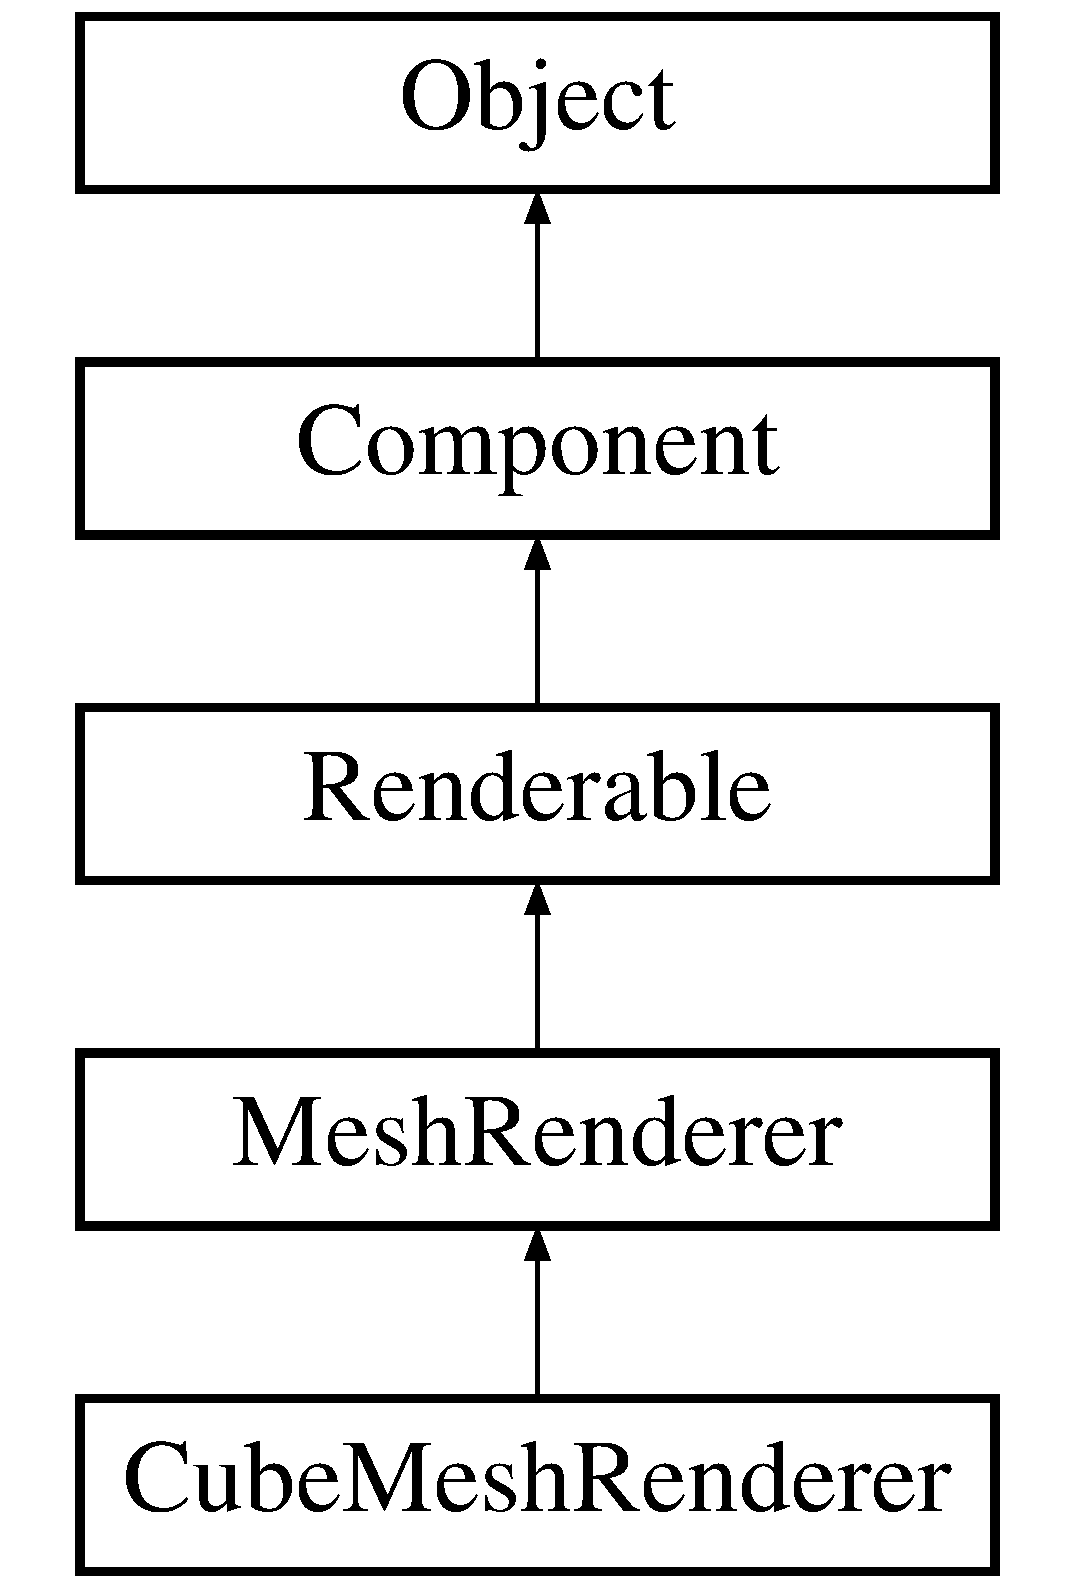
\includegraphics[height=5.000000cm]{class_cube_mesh_renderer}
\end{center}
\end{figure}
\subsection*{Public Member Functions}
\begin{DoxyCompactItemize}
\item 
\hypertarget{class_cube_mesh_renderer_a70a84151a1571740c56c4ec07a2d45b6}{
virtual const \hyperlink{class_r_t_t_i}{RTTI} \& {\bfseries getType} () const }
\label{class_cube_mesh_renderer_a70a84151a1571740c56c4ec07a2d45b6}

\item 
\hypertarget{class_cube_mesh_renderer_a637b63af1c3e8dfb8522750c406643dd}{
void {\bfseries render} () const }
\label{class_cube_mesh_renderer_a637b63af1c3e8dfb8522750c406643dd}

\end{DoxyCompactItemize}
\subsection*{Static Public Attributes}
\begin{DoxyCompactItemize}
\item 
\hypertarget{class_cube_mesh_renderer_ad25041de79d485752808bd7cd9b26a49}{
static const \hyperlink{class_r_t_t_i}{RTTI} {\bfseries TYPE}}
\label{class_cube_mesh_renderer_ad25041de79d485752808bd7cd9b26a49}

\end{DoxyCompactItemize}
\subsection*{Friends}
\begin{DoxyCompactItemize}
\item 
\hypertarget{class_cube_mesh_renderer_ac98d07dd8f7b70e16ccb9a01abf56b9c}{
class {\bfseries boost::serialization::access}}
\label{class_cube_mesh_renderer_ac98d07dd8f7b70e16ccb9a01abf56b9c}

\end{DoxyCompactItemize}


The documentation for this class was generated from the following files:\begin{DoxyCompactItemize}
\item 
CubeMeshRenderer.h\item 
CubeMeshRenderer.cpp\end{DoxyCompactItemize}

\input{class_debug_camera}
\hypertarget{class_game_object}{
\section{GameObject Class Reference}
\label{class_game_object}\index{GameObject@{GameObject}}
}
Inheritance diagram for GameObject:\begin{figure}[H]
\begin{center}
\leavevmode
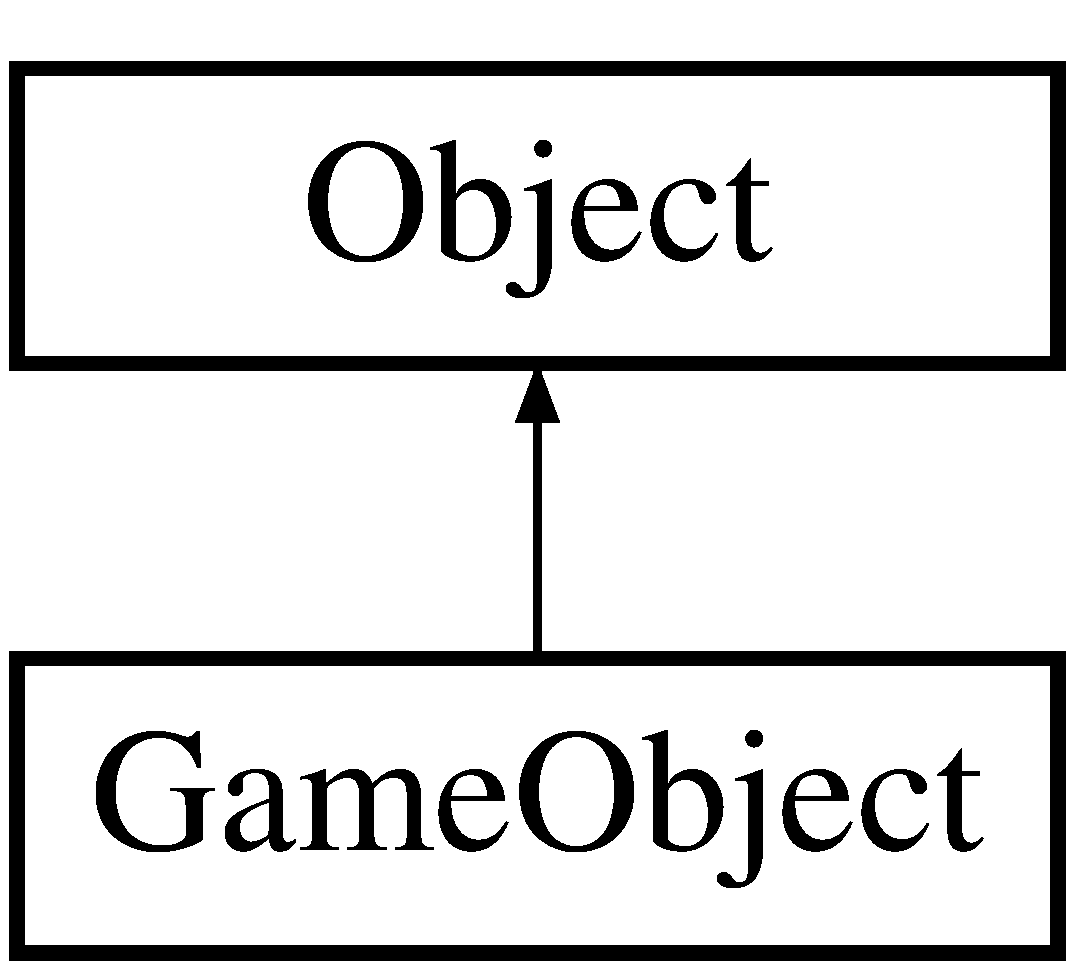
\includegraphics[height=2.000000cm]{class_game_object}
\end{center}
\end{figure}
\subsection*{Public Member Functions}
\begin{DoxyCompactItemize}
\item 
\hypertarget{class_game_object_a9286ea0f6126aca576772c7370e70d21}{
virtual const \hyperlink{class_r_t_t_i}{RTTI} \& {\bfseries getType} () const }
\label{class_game_object_a9286ea0f6126aca576772c7370e70d21}

\item 
\hypertarget{class_game_object_a8f317d59dba2a4b56b83384a94394eb8}{
void {\bfseries addComponent} (\hyperlink{class_component}{Component} $\ast$comp)}
\label{class_game_object_a8f317d59dba2a4b56b83384a94394eb8}

\item 
\hypertarget{class_game_object_a27f103522edc3f81aa62a0e9e83b5702}{
void {\bfseries setRenderer} (\hyperlink{class_renderable}{Renderable} $\ast$renderer)}
\label{class_game_object_a27f103522edc3f81aa62a0e9e83b5702}

\item 
\hypertarget{class_game_object_a3d19deea2d41be14b711ce25b65170ad}{
\hyperlink{class_renderable}{Renderable} $\ast$ {\bfseries getRenderer} () const }
\label{class_game_object_a3d19deea2d41be14b711ce25b65170ad}

\item 
\hypertarget{class_game_object_a8e76a631b7fb19c52b12d0c4b4ae9821}{
\hyperlink{class_transform}{Transform} $\ast$ {\bfseries getTransform} () const }
\label{class_game_object_a8e76a631b7fb19c52b12d0c4b4ae9821}

\item 
\hypertarget{class_game_object_a1ddc103c7b7d06748f9928f4fb378dec}{
void {\bfseries setTransform} (\hyperlink{class_transform}{Transform} $\ast$trans)}
\label{class_game_object_a1ddc103c7b7d06748f9928f4fb378dec}

\item 
\hypertarget{class_game_object_ab442beea8505007524bb1e769b9299b5}{
\hyperlink{class_behaviour}{Behaviour} $\ast$ {\bfseries getBehaviour} () const }
\label{class_game_object_ab442beea8505007524bb1e769b9299b5}

\item 
\hypertarget{class_game_object_ad84468f46d44442d784debf8dd32d43d}{
void {\bfseries setBehaviour} (\hyperlink{class_behaviour}{Behaviour} $\ast$behav)}
\label{class_game_object_ad84468f46d44442d784debf8dd32d43d}

\item 
\hypertarget{class_game_object_a98275946894e0c421675713c6fd418db}{
\hyperlink{class_collider}{Collider} $\ast$ {\bfseries getCollider} () const }
\label{class_game_object_a98275946894e0c421675713c6fd418db}

\item 
\hypertarget{class_game_object_a1c60d09ac4284c98074c91c3f2a3bd76}{
void {\bfseries setCollider} (\hyperlink{class_collider}{Collider} $\ast$collid)}
\label{class_game_object_a1c60d09ac4284c98074c91c3f2a3bd76}

\item 
\hypertarget{class_game_object_a8ee01bb9d3bf665bcdd7b01d0afa0f83}{
\hyperlink{class_animation}{Animation} $\ast$ {\bfseries getAnimation} () const }
\label{class_game_object_a8ee01bb9d3bf665bcdd7b01d0afa0f83}

\item 
\hypertarget{class_game_object_a843c29431fdc35c948d7049eea8d4a5d}{
void {\bfseries setAnimation} (\hyperlink{class_animation}{Animation} $\ast$anim)}
\label{class_game_object_a843c29431fdc35c948d7049eea8d4a5d}

\item 
\hypertarget{class_game_object_af346844a9eb537a6f5255b4af5c52439}{
\hyperlink{class_particle_system}{ParticleSystem} $\ast$ {\bfseries getParticleSystem} () const }
\label{class_game_object_af346844a9eb537a6f5255b4af5c52439}

\item 
\hypertarget{class_game_object_a3b85c8ce97b7720349707d92fc71c273}{
void {\bfseries setParticleSystem} (\hyperlink{class_particle_system}{ParticleSystem} $\ast$anim)}
\label{class_game_object_a3b85c8ce97b7720349707d92fc71c273}

\item 
\hypertarget{class_game_object_a7fddf97069213113a53d993a29255985}{
void {\bfseries onCollisionEnter} ()}
\label{class_game_object_a7fddf97069213113a53d993a29255985}

\end{DoxyCompactItemize}
\subsection*{Static Public Attributes}
\begin{DoxyCompactItemize}
\item 
\hypertarget{class_game_object_a5dce9d375b69a47b73ce1dd53bf01cc6}{
static const \hyperlink{class_r_t_t_i}{RTTI} {\bfseries TYPE}}
\label{class_game_object_a5dce9d375b69a47b73ce1dd53bf01cc6}

\end{DoxyCompactItemize}
\subsection*{Friends}
\begin{DoxyCompactItemize}
\item 
\hypertarget{class_game_object_ac98d07dd8f7b70e16ccb9a01abf56b9c}{
class {\bfseries boost::serialization::access}}
\label{class_game_object_ac98d07dd8f7b70e16ccb9a01abf56b9c}

\end{DoxyCompactItemize}


The documentation for this class was generated from the following files:\begin{DoxyCompactItemize}
\item 
GameObject.h\item 
GameObject.cpp\end{DoxyCompactItemize}

\input{class_game_object_factory}
\input{class_g_l_s_l_shader}
\input{struct_key_frame}
\hypertarget{class_light}{
\section{Light Class Reference}
\label{class_light}\index{Light@{Light}}
}
Inheritance diagram for Light:\begin{figure}[H]
\begin{center}
\leavevmode
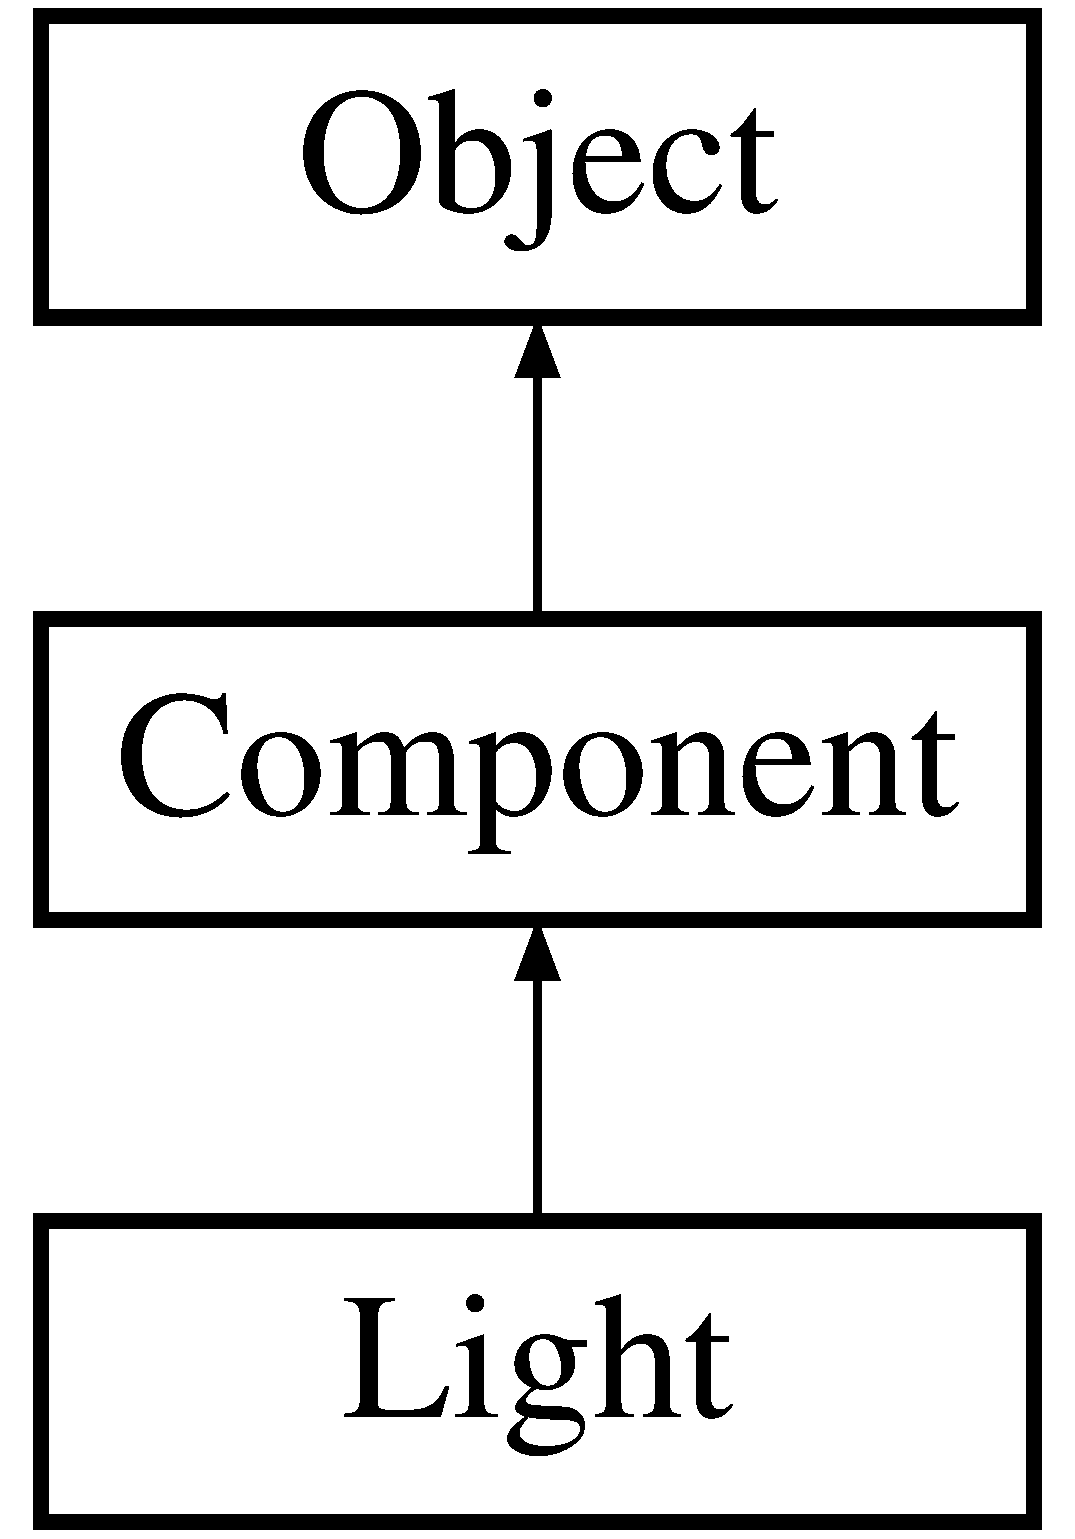
\includegraphics[height=3.000000cm]{class_light}
\end{center}
\end{figure}
\subsection*{Public Member Functions}
\begin{DoxyCompactItemize}
\item 
\hypertarget{class_light_a5404d9b1ee53f91da443c061b98a8f66}{
virtual const \hyperlink{class_r_t_t_i}{RTTI} \& {\bfseries getType} () const }
\label{class_light_a5404d9b1ee53f91da443c061b98a8f66}

\item 
\hypertarget{class_light_af5c65ad5f3237bea9f6f469eb95a66a1}{
{\bfseries Light} (const Vec4f \&amb, const Vec4f \&diff, const Vec4f \&spec, \hyperlink{class_light_manager}{LightManager} $\ast$manager)}
\label{class_light_af5c65ad5f3237bea9f6f469eb95a66a1}

\item 
\hypertarget{class_light_a45f84b6f75a0d02760d3a20efaf8f83e}{
void {\bfseries setLightType} (LightTypEnum type)}
\label{class_light_a45f84b6f75a0d02760d3a20efaf8f83e}

\item 
\hypertarget{class_light_a26ececa9d5a86203fc5cd0dfa74d76b7}{
\hyperlink{class_transform}{Transform} $\ast$ {\bfseries getTransform} () const }
\label{class_light_a26ececa9d5a86203fc5cd0dfa74d76b7}

\item 
\hypertarget{class_light_a03628bf455079a5efd55d3b2b650ff9a}{
void {\bfseries setTransform} (\hyperlink{class_transform}{Transform} $\ast$trans)}
\label{class_light_a03628bf455079a5efd55d3b2b650ff9a}

\item 
\hypertarget{class_light_a0136c2fa693d47f86c51e643b9c0a6ee}{
void {\bfseries applyLightState} ()}
\label{class_light_a0136c2fa693d47f86c51e643b9c0a6ee}

\end{DoxyCompactItemize}
\subsection*{Static Public Member Functions}
\begin{DoxyCompactItemize}
\item 
\hypertarget{class_light_a73b5878b0115b283ae5b0a82cc827dac}{
static \hyperlink{class_light}{Light} {\bfseries ambientLight} (const Vec4f \&amb, \hyperlink{class_light_manager}{LightManager} $\ast$manager)}
\label{class_light_a73b5878b0115b283ae5b0a82cc827dac}

\end{DoxyCompactItemize}
\subsection*{Static Public Attributes}
\begin{DoxyCompactItemize}
\item 
\hypertarget{class_light_a6a4b7875ce0fe875b9cddde551552526}{
static const \hyperlink{class_r_t_t_i}{RTTI} {\bfseries TYPE}}
\label{class_light_a6a4b7875ce0fe875b9cddde551552526}

\end{DoxyCompactItemize}
\subsection*{Protected Member Functions}
\begin{DoxyCompactItemize}
\item 
\hypertarget{class_light_aec8f8df7c99076d4b165382c0f04b827}{
GLenum {\bfseries intToGlLightId} (int id)}
\label{class_light_aec8f8df7c99076d4b165382c0f04b827}

\end{DoxyCompactItemize}
\subsection*{Protected Attributes}
\begin{DoxyCompactItemize}
\item 
\hypertarget{class_light_a1b68d4ff673ffffd8c6bb24995ccde1e}{
Vec4f {\bfseries diffuse}}
\label{class_light_a1b68d4ff673ffffd8c6bb24995ccde1e}

\item 
\hypertarget{class_light_afa8ce9cb262a986a0fee095c8420fe0a}{
Vec4f {\bfseries ambient}}
\label{class_light_afa8ce9cb262a986a0fee095c8420fe0a}

\item 
\hypertarget{class_light_a0e4f7cb1501e06372a016e9264db37c8}{
Vec4f {\bfseries specular}}
\label{class_light_a0e4f7cb1501e06372a016e9264db37c8}

\item 
\hypertarget{class_light_a5c02ae068c634bf7327e4b66b4ea8744}{
float {\bfseries coneAngle}}
\label{class_light_a5c02ae068c634bf7327e4b66b4ea8744}

\item 
\hypertarget{class_light_a0f24e5db8e0b914a745c0a0f5bbef1f6}{
float {\bfseries coneExponent}}
\label{class_light_a0f24e5db8e0b914a745c0a0f5bbef1f6}

\item 
\hypertarget{class_light_aa4da12007ef812f8c73b0c65b19ee501}{
LightTypEnum {\bfseries lightType}}
\label{class_light_aa4da12007ef812f8c73b0c65b19ee501}

\item 
\hypertarget{class_light_a2dd418642e49db9b22bd206c82a8f29a}{
GLenum {\bfseries glLightId}}
\label{class_light_a2dd418642e49db9b22bd206c82a8f29a}

\item 
\hypertarget{class_light_a23c44b0fcf2249ff53707d136a2cfdc4}{
\hyperlink{class_transform}{Transform} $\ast$ {\bfseries transform}}
\label{class_light_a23c44b0fcf2249ff53707d136a2cfdc4}

\end{DoxyCompactItemize}


The documentation for this class was generated from the following files:\begin{DoxyCompactItemize}
\item 
Light.h\item 
Light.cpp\end{DoxyCompactItemize}

\hypertarget{class_light_factory}{
\section{LightFactory Class Reference}
\label{class_light_factory}\index{LightFactory@{LightFactory}}
}
\subsection*{Protected Attributes}
\begin{DoxyCompactItemize}
\item 
\hypertarget{class_light_factory_a7f4e30200f477d6dff387f0ff172fa4c}{
int {\bfseries numberOfLights}}
\label{class_light_factory_a7f4e30200f477d6dff387f0ff172fa4c}

\end{DoxyCompactItemize}


The documentation for this class was generated from the following files:\begin{DoxyCompactItemize}
\item 
LightFactory.h\item 
LightFactory.cpp\end{DoxyCompactItemize}

\hypertarget{class_light_manager}{
\section{LightManager Class Reference}
\label{class_light_manager}\index{LightManager@{LightManager}}
}
\subsection*{Public Member Functions}
\begin{DoxyCompactItemize}
\item 
\hypertarget{class_light_manager_a0e9df103ca3061304962a734c63a3749}{
int {\bfseries getAvailableLightId} ()}
\label{class_light_manager_a0e9df103ca3061304962a734c63a3749}

\end{DoxyCompactItemize}
\subsection*{Static Public Member Functions}
\begin{DoxyCompactItemize}
\item 
\hypertarget{class_light_manager_a173a4cfc7bc844e10a02be0d4dab00c9}{
static \hyperlink{class_light_manager}{LightManager} $\ast$ {\bfseries getInstance} ()}
\label{class_light_manager_a173a4cfc7bc844e10a02be0d4dab00c9}

\end{DoxyCompactItemize}


The documentation for this class was generated from the following files:\begin{DoxyCompactItemize}
\item 
LightManager.h\item 
LightManager.cpp\end{DoxyCompactItemize}

\hypertarget{class_material}{
\section{Material Class Reference}
\label{class_material}\index{Material@{Material}}
}
Inheritance diagram for Material:\begin{figure}[H]
\begin{center}
\leavevmode
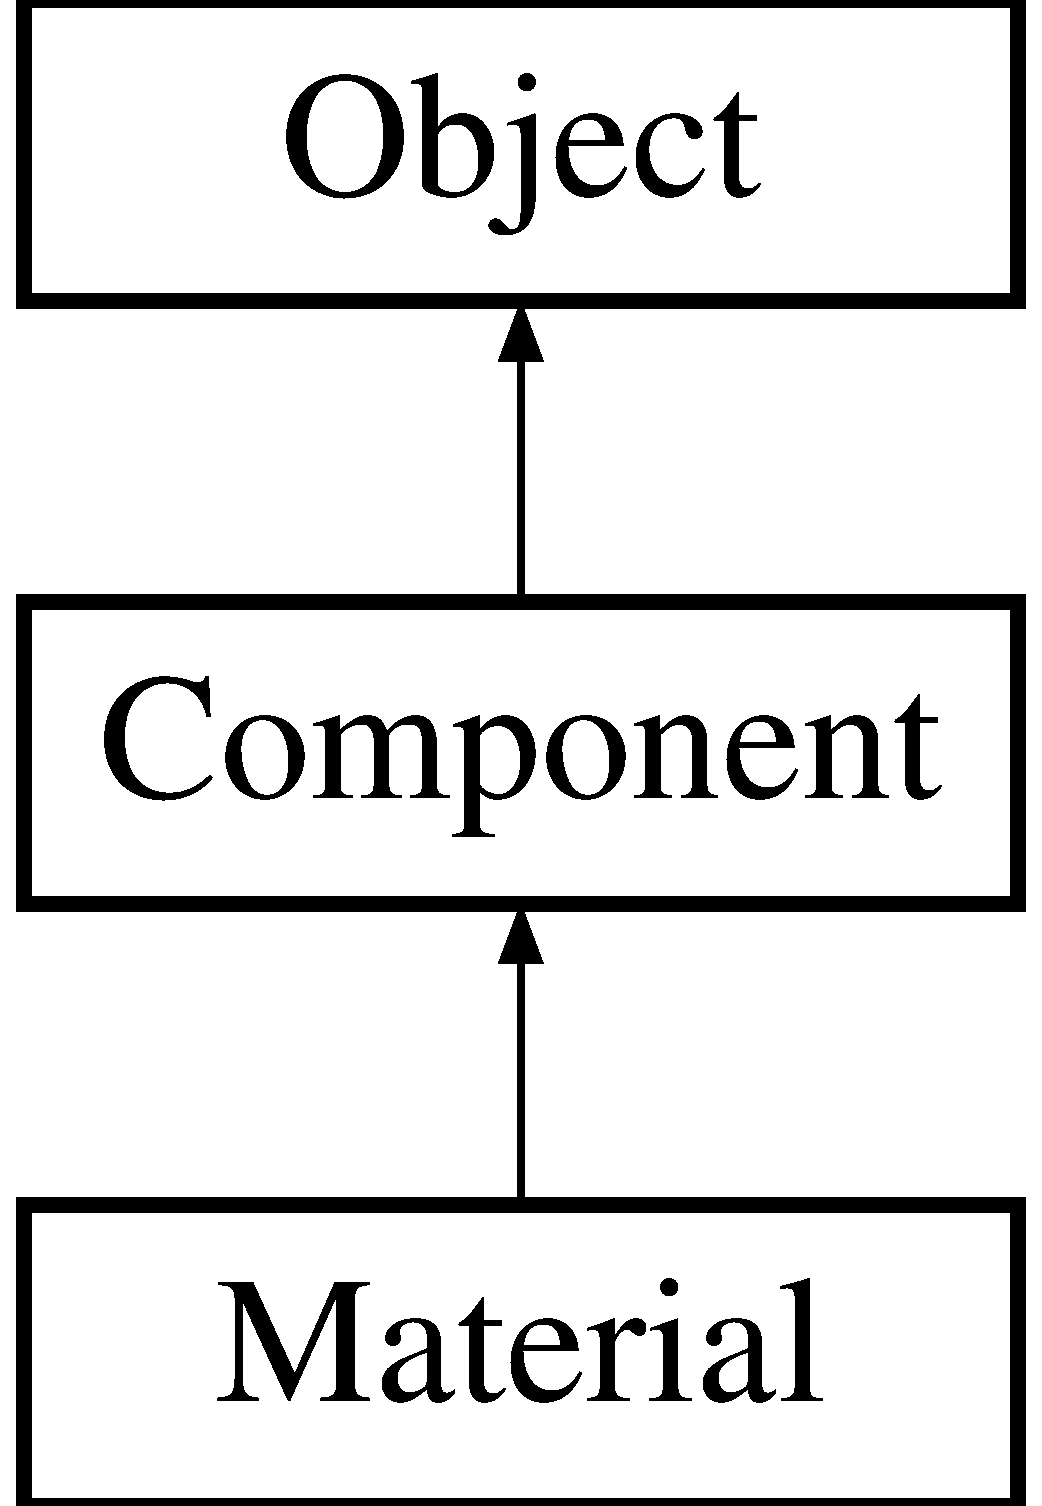
\includegraphics[height=3.000000cm]{class_material}
\end{center}
\end{figure}
\subsection*{Public Member Functions}
\begin{DoxyCompactItemize}
\item 
\hypertarget{class_material_a1acc2b274cb26a7596d7ad431d44a85b}{
virtual const \hyperlink{class_r_t_t_i}{RTTI} \& {\bfseries getType} () const }
\label{class_material_a1acc2b274cb26a7596d7ad431d44a85b}

\item 
\hypertarget{class_material_a85bc5c4fadca145531972bc2238a62fa}{
{\bfseries Material} (ColorEnum Color)}
\label{class_material_a85bc5c4fadca145531972bc2238a62fa}

\item 
\hypertarget{class_material_a2b1512217db95dca5fb753244f942fe5}{
{\bfseries Material} (const Vec4f \&Color)}
\label{class_material_a2b1512217db95dca5fb753244f942fe5}

\item 
\hypertarget{class_material_af5b80bf73b7ea87a3d9d3855596be1f4}{
void {\bfseries setTexture} (\hyperlink{class_texture}{Texture} $\ast$tex)}
\label{class_material_af5b80bf73b7ea87a3d9d3855596be1f4}

\item 
\hypertarget{class_material_a3f618cc74964d2e3af42b843d5d4527b}{
void {\bfseries setShader} (\hyperlink{class_g_l_s_l_shader}{GLSLShader} $\ast$Shader)}
\label{class_material_a3f618cc74964d2e3af42b843d5d4527b}

\item 
\hypertarget{class_material_a0c1158aadbd8a977a59befef87310cb5}{
void {\bfseries setMaterialState} (bool receives\_\-shadow) const }
\label{class_material_a0c1158aadbd8a977a59befef87310cb5}

\end{DoxyCompactItemize}
\subsection*{Static Public Attributes}
\begin{DoxyCompactItemize}
\item 
\hypertarget{class_material_a2ce292caf29777172f41f1e2cfa3f4de}{
static const \hyperlink{class_r_t_t_i}{RTTI} {\bfseries TYPE}}
\label{class_material_a2ce292caf29777172f41f1e2cfa3f4de}

\end{DoxyCompactItemize}
\subsection*{Friends}
\begin{DoxyCompactItemize}
\item 
\hypertarget{class_material_ac98d07dd8f7b70e16ccb9a01abf56b9c}{
class {\bfseries boost::serialization::access}}
\label{class_material_ac98d07dd8f7b70e16ccb9a01abf56b9c}

\end{DoxyCompactItemize}


The documentation for this class was generated from the following files:\begin{DoxyCompactItemize}
\item 
Material.h\item 
Material.cpp\end{DoxyCompactItemize}

\hypertarget{class_mesh_renderer}{
\section{MeshRenderer Class Reference}
\label{class_mesh_renderer}\index{MeshRenderer@{MeshRenderer}}
}
Inheritance diagram for MeshRenderer:\begin{figure}[H]
\begin{center}
\leavevmode
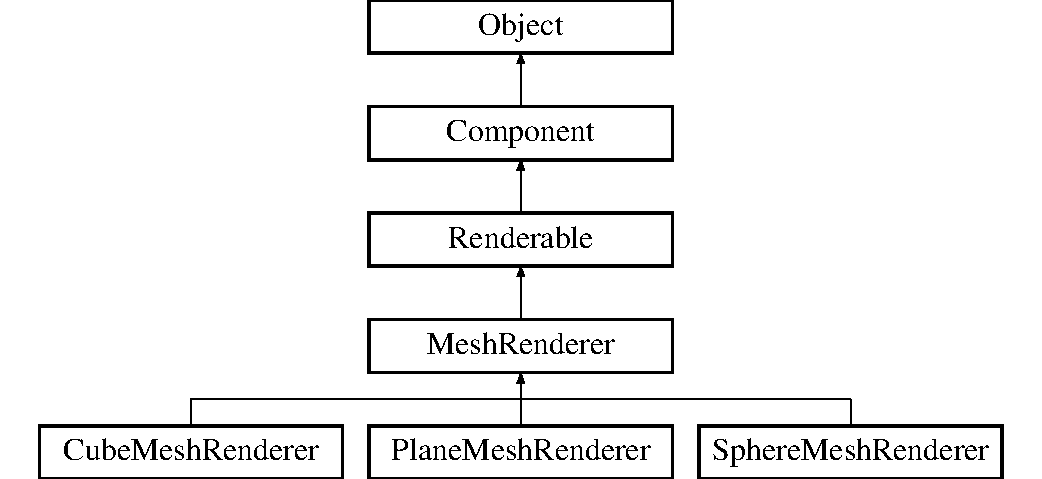
\includegraphics[height=5.000000cm]{class_mesh_renderer}
\end{center}
\end{figure}
\subsection*{Public Member Functions}
\begin{DoxyCompactItemize}
\item 
\hypertarget{class_mesh_renderer_a4430f795bd67ba8aca7b57bab488971b}{
virtual const \hyperlink{class_r_t_t_i}{RTTI} \& {\bfseries getType} () const }
\label{class_mesh_renderer_a4430f795bd67ba8aca7b57bab488971b}

\item 
\hypertarget{class_mesh_renderer_a81dd19d7a59f2d8bb086ab939b19a4c5}{
{\bfseries MeshRenderer} (BasicShapeEnum shape)}
\label{class_mesh_renderer_a81dd19d7a59f2d8bb086ab939b19a4c5}

\item 
\hypertarget{class_mesh_renderer_a5a811c3fbbdd31edef0ef23c3219c35e}{
virtual void {\bfseries render} () const }
\label{class_mesh_renderer_a5a811c3fbbdd31edef0ef23c3219c35e}

\item 
\hypertarget{class_mesh_renderer_ae7f66301b96360025adbd901465ef9d5}{
void {\bfseries setMaterial} (\hyperlink{class_material}{Material} $\ast$)}
\label{class_mesh_renderer_ae7f66301b96360025adbd901465ef9d5}

\item 
\hypertarget{class_mesh_renderer_a75c264da40ce0ac85919736c2905203e}{
\hyperlink{class_material}{Material} $\ast$ {\bfseries getMaterial} ()}
\label{class_mesh_renderer_a75c264da40ce0ac85919736c2905203e}

\item 
\hypertarget{class_mesh_renderer_a16a30a96dccb8b557247322e247d4a8f}{
void {\bfseries setMesh} (\hyperlink{class_t_r3_d_1_1_tri_mesh}{TriMesh} $\ast$Mesh)}
\label{class_mesh_renderer_a16a30a96dccb8b557247322e247d4a8f}

\item 
\hypertarget{class_mesh_renderer_ab66e3b92d702f2b93d3d3afb74807d24}{
\hyperlink{class_t_r3_d_1_1_tri_mesh}{TriMesh} $\ast$ {\bfseries getMesh} ()}
\label{class_mesh_renderer_ab66e3b92d702f2b93d3d3afb74807d24}

\item 
\hypertarget{class_mesh_renderer_a18e4146b5a29d4916dca693f39db2233}{
bool {\bfseries castShadow} () const }
\label{class_mesh_renderer_a18e4146b5a29d4916dca693f39db2233}

\item 
\hypertarget{class_mesh_renderer_ac150da9be57d1616c1a5ccba374fa2fb}{
bool {\bfseries receiveShadow} () const }
\label{class_mesh_renderer_ac150da9be57d1616c1a5ccba374fa2fb}

\item 
\hypertarget{class_mesh_renderer_a58101967c2a4cd65513aeb4b940314ec}{
void {\bfseries setCastShadow} (bool cast)}
\label{class_mesh_renderer_a58101967c2a4cd65513aeb4b940314ec}

\item 
\hypertarget{class_mesh_renderer_abf4aa0764b41e79388905f6c23457d00}{
void {\bfseries setReceiveShadow} (bool receive)}
\label{class_mesh_renderer_abf4aa0764b41e79388905f6c23457d00}

\end{DoxyCompactItemize}
\subsection*{Static Public Attributes}
\begin{DoxyCompactItemize}
\item 
\hypertarget{class_mesh_renderer_af9376b762b4c96f9e92ebb3bf94458df}{
static const \hyperlink{class_r_t_t_i}{RTTI} {\bfseries TYPE}}
\label{class_mesh_renderer_af9376b762b4c96f9e92ebb3bf94458df}

\end{DoxyCompactItemize}
\subsection*{Protected Attributes}
\begin{DoxyCompactItemize}
\item 
\hypertarget{class_mesh_renderer_ae5987818b394c9677ed984fcd254fc07}{
int {\bfseries nbOfVertices}}
\label{class_mesh_renderer_ae5987818b394c9677ed984fcd254fc07}

\item 
\hypertarget{class_mesh_renderer_a35d178fce64e5ef4c07bbb59706a6b65}{
Vec3f $\ast$ {\bfseries vertices}}
\label{class_mesh_renderer_a35d178fce64e5ef4c07bbb59706a6b65}

\item 
\hypertarget{class_mesh_renderer_a18547492a62a887bc63ae950ed947de7}{
Vec3f $\ast$ {\bfseries normals}}
\label{class_mesh_renderer_a18547492a62a887bc63ae950ed947de7}

\item 
\hypertarget{class_mesh_renderer_a39910329c399dcf516e9e6d3a70e4ce8}{
\hyperlink{class_material}{Material} $\ast$ {\bfseries material}}
\label{class_mesh_renderer_a39910329c399dcf516e9e6d3a70e4ce8}

\item 
\hypertarget{class_mesh_renderer_a75f70932dae889f11d5614ef46ac3d11}{
\hyperlink{class_t_r3_d_1_1_tri_mesh}{TriMesh} $\ast$ {\bfseries mesh}}
\label{class_mesh_renderer_a75f70932dae889f11d5614ef46ac3d11}

\item 
\hypertarget{class_mesh_renderer_a92a86c242532912eebf5cf7dad28e5a2}{
bool {\bfseries \_\-castShadow}}
\label{class_mesh_renderer_a92a86c242532912eebf5cf7dad28e5a2}

\item 
\hypertarget{class_mesh_renderer_a96df19ab2f11f1319803ae0aacb0a8b6}{
bool {\bfseries \_\-receiveShadow}}
\label{class_mesh_renderer_a96df19ab2f11f1319803ae0aacb0a8b6}

\end{DoxyCompactItemize}
\subsection*{Friends}
\begin{DoxyCompactItemize}
\item 
\hypertarget{class_mesh_renderer_ac98d07dd8f7b70e16ccb9a01abf56b9c}{
class {\bfseries boost::serialization::access}}
\label{class_mesh_renderer_ac98d07dd8f7b70e16ccb9a01abf56b9c}

\end{DoxyCompactItemize}


The documentation for this class was generated from the following files:\begin{DoxyCompactItemize}
\item 
MeshRenderer.h\item 
MeshRenderer.cpp\end{DoxyCompactItemize}

\hypertarget{class_object}{
\section{Object Class Reference}
\label{class_object}\index{Object@{Object}}
}
Inheritance diagram for Object:\begin{figure}[H]
\begin{center}
\leavevmode
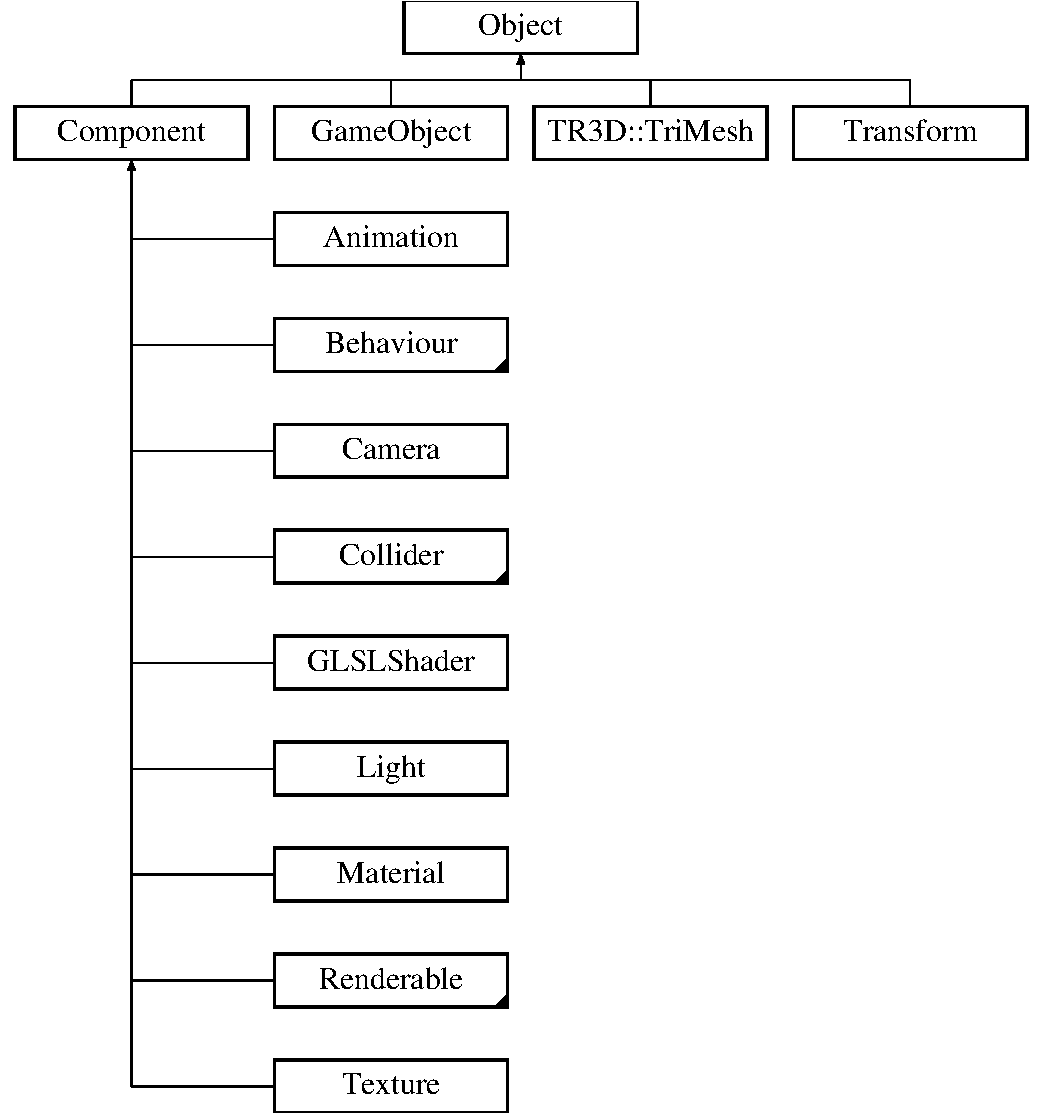
\includegraphics[height=11.000000cm]{class_object}
\end{center}
\end{figure}
\subsection*{Public Member Functions}
\begin{DoxyCompactItemize}
\item 
\hypertarget{class_object_aced0a1a622fb0155b74f6e2e1058b2c2}{
virtual const \hyperlink{class_r_t_t_i}{RTTI} \& {\bfseries getType} () const }
\label{class_object_aced0a1a622fb0155b74f6e2e1058b2c2}

\item 
\hypertarget{class_object_ab38070a3be64ec57740528011a10d542}{
{\bfseries Object} (const string \&name)}
\label{class_object_ab38070a3be64ec57740528011a10d542}

\item 
\hypertarget{class_object_a6b8fc39c7613b32e5e25e549aaf293ad}{
void {\bfseries setName} (const string \&name)}
\label{class_object_a6b8fc39c7613b32e5e25e549aaf293ad}

\item 
\hypertarget{class_object_a40651ab63aba5bfb7ddc6f495d5d4b60}{
const string \& {\bfseries getName} () const }
\label{class_object_a40651ab63aba5bfb7ddc6f495d5d4b60}

\item 
\hypertarget{class_object_a870ac8cc97fa1d18b1a503c9a9245895}{
void {\bfseries incRef} ()}
\label{class_object_a870ac8cc97fa1d18b1a503c9a9245895}

\item 
\hypertarget{class_object_a164b1855548a10e8881f3bef5ad9d917}{
void {\bfseries decRef} ()}
\label{class_object_a164b1855548a10e8881f3bef5ad9d917}

\item 
\hypertarget{class_object_ad5037099674461f49304cfe2d26ef317}{
int {\bfseries getRefCount} () const }
\label{class_object_ad5037099674461f49304cfe2d26ef317}

\end{DoxyCompactItemize}
\subsection*{Static Public Attributes}
\begin{DoxyCompactItemize}
\item 
\hypertarget{class_object_a5e2bc03cb3fa6122b28fff1b0049a30e}{
static const \hyperlink{class_r_t_t_i}{RTTI} {\bfseries TYPE}}
\label{class_object_a5e2bc03cb3fa6122b28fff1b0049a30e}

\end{DoxyCompactItemize}
\subsection*{Protected Attributes}
\begin{DoxyCompactItemize}
\item 
\hypertarget{class_object_a45e76e41e7fa83161a09c5694088a3bf}{
unsigned int {\bfseries id}}
\label{class_object_a45e76e41e7fa83161a09c5694088a3bf}

\item 
\hypertarget{class_object_af849c7778ff8399ac4440062ac5a38a3}{
string {\bfseries name}}
\label{class_object_af849c7778ff8399ac4440062ac5a38a3}

\end{DoxyCompactItemize}
\subsection*{Friends}
\begin{DoxyCompactItemize}
\item 
\hypertarget{class_object_ac98d07dd8f7b70e16ccb9a01abf56b9c}{
class {\bfseries boost::serialization::access}}
\label{class_object_ac98d07dd8f7b70e16ccb9a01abf56b9c}

\end{DoxyCompactItemize}


The documentation for this class was generated from the following files:\begin{DoxyCompactItemize}
\item 
Object.h\item 
Object.cpp\end{DoxyCompactItemize}

\input{class_particle_system}
\input{class_plane_collider}
\hypertarget{class_plane_mesh_renderer}{
\section{PlaneMeshRenderer Class Reference}
\label{class_plane_mesh_renderer}\index{PlaneMeshRenderer@{PlaneMeshRenderer}}
}
Inheritance diagram for PlaneMeshRenderer:\begin{figure}[H]
\begin{center}
\leavevmode
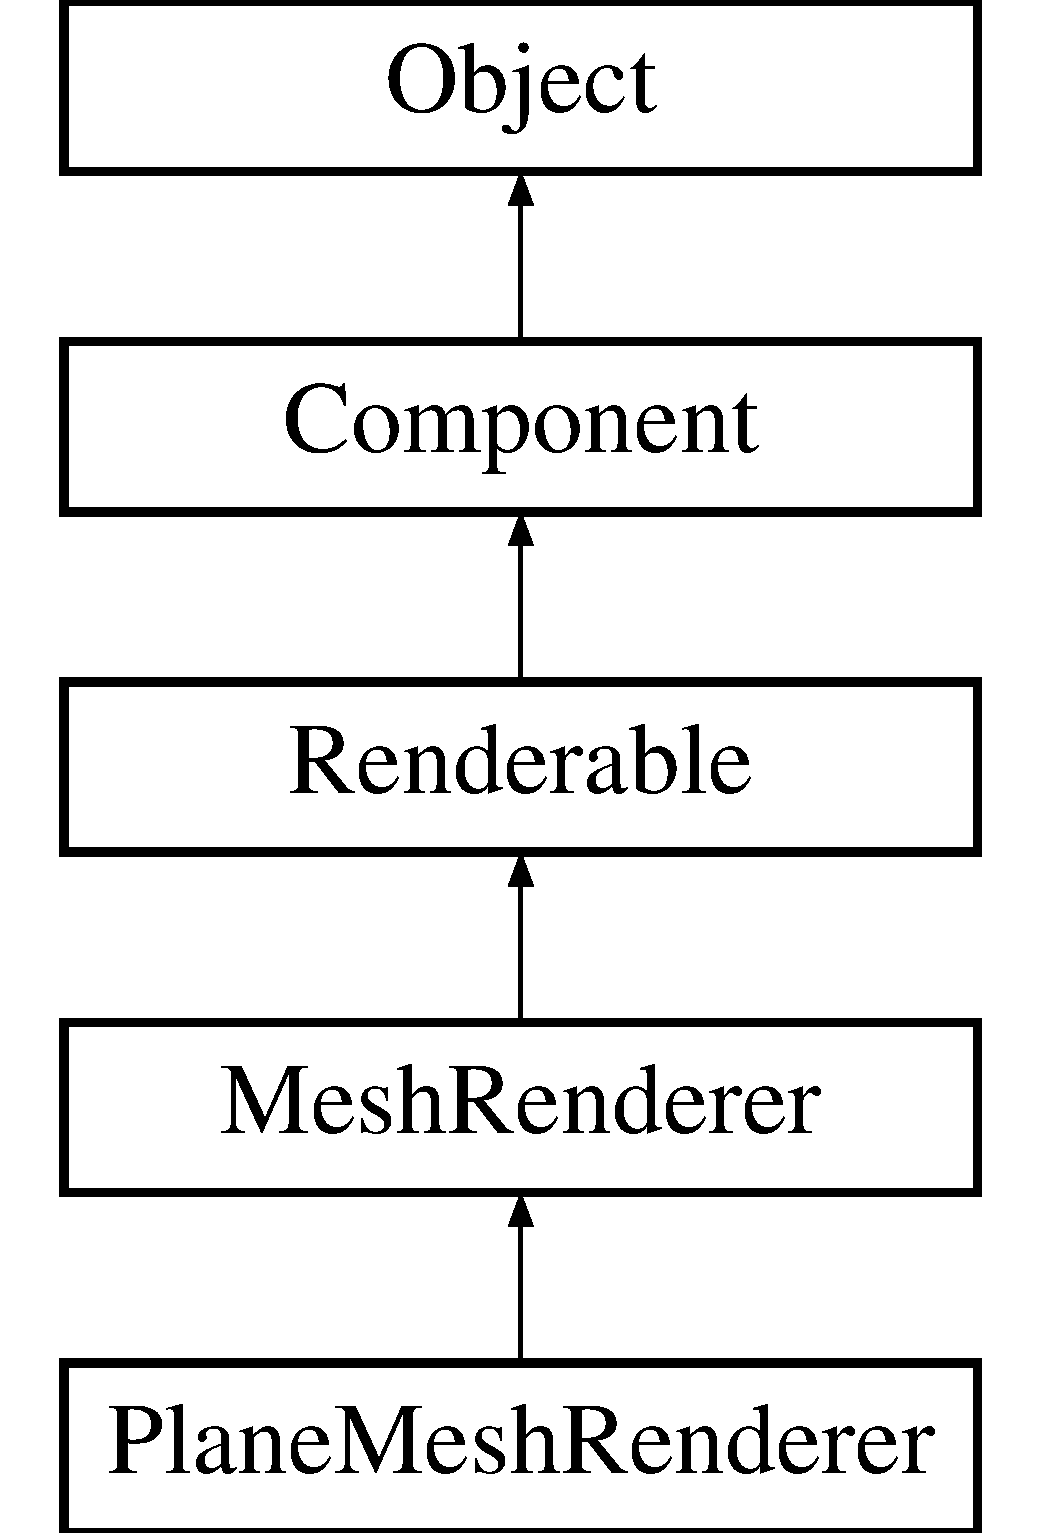
\includegraphics[height=5.000000cm]{class_plane_mesh_renderer}
\end{center}
\end{figure}
\subsection*{Public Member Functions}
\begin{DoxyCompactItemize}
\item 
\hypertarget{class_plane_mesh_renderer_a9253e40492fe5d345b4d3ff809943dcc}{
virtual const \hyperlink{class_r_t_t_i}{RTTI} \& {\bfseries getType} () const }
\label{class_plane_mesh_renderer_a9253e40492fe5d345b4d3ff809943dcc}

\item 
\hypertarget{class_plane_mesh_renderer_a61d0cf9da44ea7de4ca60552edc82790}{
void {\bfseries render} () const }
\label{class_plane_mesh_renderer_a61d0cf9da44ea7de4ca60552edc82790}

\end{DoxyCompactItemize}
\subsection*{Static Public Attributes}
\begin{DoxyCompactItemize}
\item 
\hypertarget{class_plane_mesh_renderer_adaea4ffb672549bb4f152748f465ba4a}{
static const \hyperlink{class_r_t_t_i}{RTTI} {\bfseries TYPE}}
\label{class_plane_mesh_renderer_adaea4ffb672549bb4f152748f465ba4a}

\end{DoxyCompactItemize}
\subsection*{Friends}
\begin{DoxyCompactItemize}
\item 
\hypertarget{class_plane_mesh_renderer_ac98d07dd8f7b70e16ccb9a01abf56b9c}{
class {\bfseries boost::serialization::access}}
\label{class_plane_mesh_renderer_ac98d07dd8f7b70e16ccb9a01abf56b9c}

\end{DoxyCompactItemize}


The documentation for this class was generated from the following files:\begin{DoxyCompactItemize}
\item 
PlaneMeshRenderer.h\item 
PlaneMeshRenderer.cpp\end{DoxyCompactItemize}

\input{class_pointer}
\input{struct_ray}
\input{struct_ray_cast_hit}
\input{class_renderable}
\input{class_ressource}
\input{class_ressource_manager}
\input{class_r_t_t_i}
\hypertarget{class_scene}{
\section{Scene Class Reference}
\label{class_scene}\index{Scene@{Scene}}
}
\subsection*{Public Member Functions}
\begin{DoxyCompactItemize}
\item 
\hypertarget{class_scene_a4ddf2d16f371ee9533b3faf1dd5ddfb1}{
void {\bfseries render} ()}
\label{class_scene_a4ddf2d16f371ee9533b3faf1dd5ddfb1}

\item 
\hypertarget{class_scene_a69f2b1c4849bc11d64820473d0346055}{
void {\bfseries setRoot} (\hyperlink{class_transform}{Transform} $\ast$root)}
\label{class_scene_a69f2b1c4849bc11d64820473d0346055}

\item 
\hypertarget{class_scene_a47f1c7d12d5a8579d798e03d7b046a5c}{
\hyperlink{class_transform}{Transform} $\ast$ {\bfseries getRoot} ()}
\label{class_scene_a47f1c7d12d5a8579d798e03d7b046a5c}

\item 
\hypertarget{class_scene_a6320c8939cde42065e446ec96fb773ac}{
void {\bfseries addGameObject} (\hyperlink{class_game_object}{GameObject} $\ast$object)}
\label{class_scene_a6320c8939cde42065e446ec96fb773ac}

\item 
\hypertarget{class_scene_a6c25f42faa6ce62b9aa2ecf97ef92447}{
void {\bfseries removeGameObject} (\hyperlink{class_game_object}{GameObject} $\ast$object)}
\label{class_scene_a6c25f42faa6ce62b9aa2ecf97ef92447}

\item 
\hypertarget{class_scene_a13b298b0c24c92929bf9850012980623}{
void {\bfseries addLight} (\hyperlink{class_light}{Light} $\ast$light)}
\label{class_scene_a13b298b0c24c92929bf9850012980623}

\item 
\hypertarget{class_scene_a41cdd9b48a474cc640ae00a84188e81a}{
void {\bfseries addMeshRenderer} (\hyperlink{class_mesh_renderer}{MeshRenderer} $\ast$renderer)}
\label{class_scene_a41cdd9b48a474cc640ae00a84188e81a}

\item 
\hypertarget{class_scene_a02f79812e48581675c97c67c598fbe9b}{
void {\bfseries applyLightsStates} () const }
\label{class_scene_a02f79812e48581675c97c67c598fbe9b}

\item 
\hypertarget{class_scene_a5cbb688a0217639bcc285c01fa005af9}{
void {\bfseries addCamera} (\hyperlink{class_camera}{Camera} $\ast$camera)}
\label{class_scene_a5cbb688a0217639bcc285c01fa005af9}

\item 
\hypertarget{class_scene_aa7a931a7e530c936433c3950c07f797e}{
void {\bfseries setMainCamera} (\hyperlink{class_camera}{Camera} $\ast$camera)}
\label{class_scene_aa7a931a7e530c936433c3950c07f797e}

\item 
\hypertarget{class_scene_a7da13a9b6cdc118cee47666ad164380d}{
void {\bfseries updateRenderQueue} ()}
\label{class_scene_a7da13a9b6cdc118cee47666ad164380d}

\end{DoxyCompactItemize}
\subsection*{Static Public Member Functions}
\begin{DoxyCompactItemize}
\item 
\hypertarget{class_scene_a18d706b52a631806605de9271f634cda}{
static void {\bfseries printNode} (\hyperlink{class_transform}{Transform} $\ast$trans, int level=0)}
\label{class_scene_a18d706b52a631806605de9271f634cda}

\item 
\hypertarget{class_scene_a0c564ec7ac34966a1cc1ceb0a4bf89ad}{
static void {\bfseries printSceneInfo} (\hyperlink{class_scene}{Scene} $\ast$scene)}
\label{class_scene_a0c564ec7ac34966a1cc1ceb0a4bf89ad}

\end{DoxyCompactItemize}
\subsection*{Static Public Attributes}
\begin{DoxyCompactItemize}
\item 
\hypertarget{class_scene_ae8c9fdb61e1c4575d04054bdd22465ff}{
static GLuint {\bfseries shadowMap} = 0}
\label{class_scene_ae8c9fdb61e1c4575d04054bdd22465ff}

\item 
\hypertarget{class_scene_a08b50d77587fb485b7a46dc4bd62002b}{
static Mat4x4f {\bfseries projShadowMatrix} = Mat4x4f(0)}
\label{class_scene_a08b50d77587fb485b7a46dc4bd62002b}

\end{DoxyCompactItemize}
\subsection*{Protected Member Functions}
\begin{DoxyCompactItemize}
\item 
\hypertarget{class_scene_a51c2c0fbc037c46049e4dc48567c17bb}{
void {\bfseries traverseSceneGraph} ()}
\label{class_scene_a51c2c0fbc037c46049e4dc48567c17bb}

\item 
\hypertarget{class_scene_a8325c012e9d12ca4afe9b50aaeecb4a1}{
void {\bfseries make\_\-proj\_\-shadow\_\-texture} (\hyperlink{class_light}{Light} $\ast$light)}
\label{class_scene_a8325c012e9d12ca4afe9b50aaeecb4a1}

\end{DoxyCompactItemize}
\subsection*{Protected Attributes}
\begin{DoxyCompactItemize}
\item 
\hypertarget{class_scene_a4010430ecd2e23c7d96764e6fdacb1a6}{
std::vector$<$ \hyperlink{class_transform}{Transform} $\ast$ $>$ {\bfseries transforms}}
\label{class_scene_a4010430ecd2e23c7d96764e6fdacb1a6}

\item 
\hypertarget{class_scene_a4ecc3182a80435e1c4dfbe1b20e559bd}{
std::vector$<$ \hyperlink{class_light}{Light} $\ast$ $>$ {\bfseries lights}}
\label{class_scene_a4ecc3182a80435e1c4dfbe1b20e559bd}

\item 
\hypertarget{class_scene_a766a660b1b9d851b14157a6d9373f719}{
std::vector$<$ \hyperlink{class_camera}{Camera} $\ast$ $>$ {\bfseries cameras}}
\label{class_scene_a766a660b1b9d851b14157a6d9373f719}

\item 
\hypertarget{class_scene_a38d0a48c9b531a3012bbb14f0455ddf0}{
std::vector$<$ \hyperlink{class_renderable}{Renderable} $\ast$ $>$ {\bfseries renderQueue}}
\label{class_scene_a38d0a48c9b531a3012bbb14f0455ddf0}

\item 
\hypertarget{class_scene_ac40b87dab6f00fa2ad4819c52559d699}{
std::vector$<$ \hyperlink{class_renderable}{Renderable} $\ast$ $>$ {\bfseries shadowCasters}}
\label{class_scene_ac40b87dab6f00fa2ad4819c52559d699}

\item 
\hypertarget{class_scene_ad9ed8db8f6868234e789557e267cc2e7}{
\hyperlink{class_transform}{Transform} $\ast$ {\bfseries sceneRoot}}
\label{class_scene_ad9ed8db8f6868234e789557e267cc2e7}

\item 
\hypertarget{class_scene_a878011b448f85714694abf6ddeee9376}{
\hyperlink{class_camera}{Camera} $\ast$ {\bfseries mainCamera}}
\label{class_scene_a878011b448f85714694abf6ddeee9376}

\end{DoxyCompactItemize}


The documentation for this class was generated from the following files:\begin{DoxyCompactItemize}
\item 
Scene.h\item 
Scene.cpp\end{DoxyCompactItemize}

\input{class_screen}
\input{class_sphere_collider}
\hypertarget{class_sphere_mesh_renderer}{
\section{SphereMeshRenderer Class Reference}
\label{class_sphere_mesh_renderer}\index{SphereMeshRenderer@{SphereMeshRenderer}}
}
Inheritance diagram for SphereMeshRenderer:\begin{figure}[H]
\begin{center}
\leavevmode
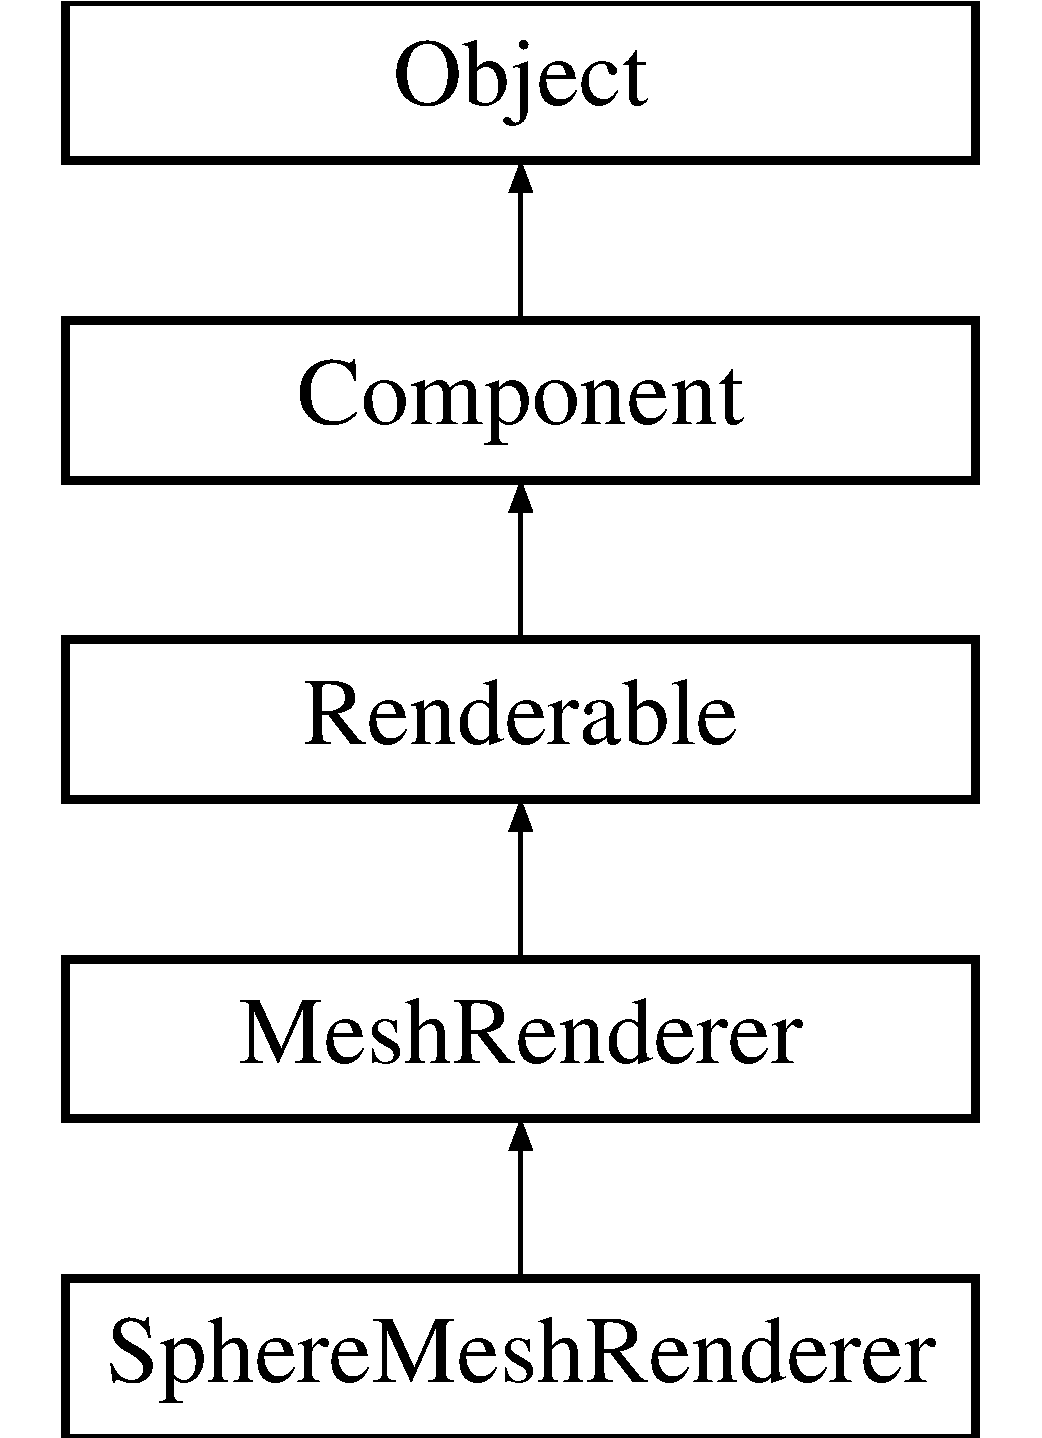
\includegraphics[height=5.000000cm]{class_sphere_mesh_renderer}
\end{center}
\end{figure}
\subsection*{Public Member Functions}
\begin{DoxyCompactItemize}
\item 
\hypertarget{class_sphere_mesh_renderer_a74dd0471e210aee688fa2239030a2ef2}{
virtual const \hyperlink{class_r_t_t_i}{RTTI} \& {\bfseries getType} () const }
\label{class_sphere_mesh_renderer_a74dd0471e210aee688fa2239030a2ef2}

\item 
\hypertarget{class_sphere_mesh_renderer_a1a000a113c48518c519873ff214a60fb}{
void {\bfseries render} () const }
\label{class_sphere_mesh_renderer_a1a000a113c48518c519873ff214a60fb}

\end{DoxyCompactItemize}
\subsection*{Static Public Attributes}
\begin{DoxyCompactItemize}
\item 
\hypertarget{class_sphere_mesh_renderer_a14b09908d23ee74b4086c9428b621584}{
static const \hyperlink{class_r_t_t_i}{RTTI} {\bfseries TYPE}}
\label{class_sphere_mesh_renderer_a14b09908d23ee74b4086c9428b621584}

\end{DoxyCompactItemize}
\subsection*{Friends}
\begin{DoxyCompactItemize}
\item 
\hypertarget{class_sphere_mesh_renderer_ac98d07dd8f7b70e16ccb9a01abf56b9c}{
class {\bfseries boost::serialization::access}}
\label{class_sphere_mesh_renderer_ac98d07dd8f7b70e16ccb9a01abf56b9c}

\end{DoxyCompactItemize}


The documentation for this class was generated from the following files:\begin{DoxyCompactItemize}
\item 
SphereMeshRenderer.h\item 
SphereMeshRenderer.cpp\end{DoxyCompactItemize}

\input{class_terrain}
\hypertarget{class_texture}{
\section{Texture Class Reference}
\label{class_texture}\index{Texture@{Texture}}
}
Inheritance diagram for Texture:\begin{figure}[H]
\begin{center}
\leavevmode
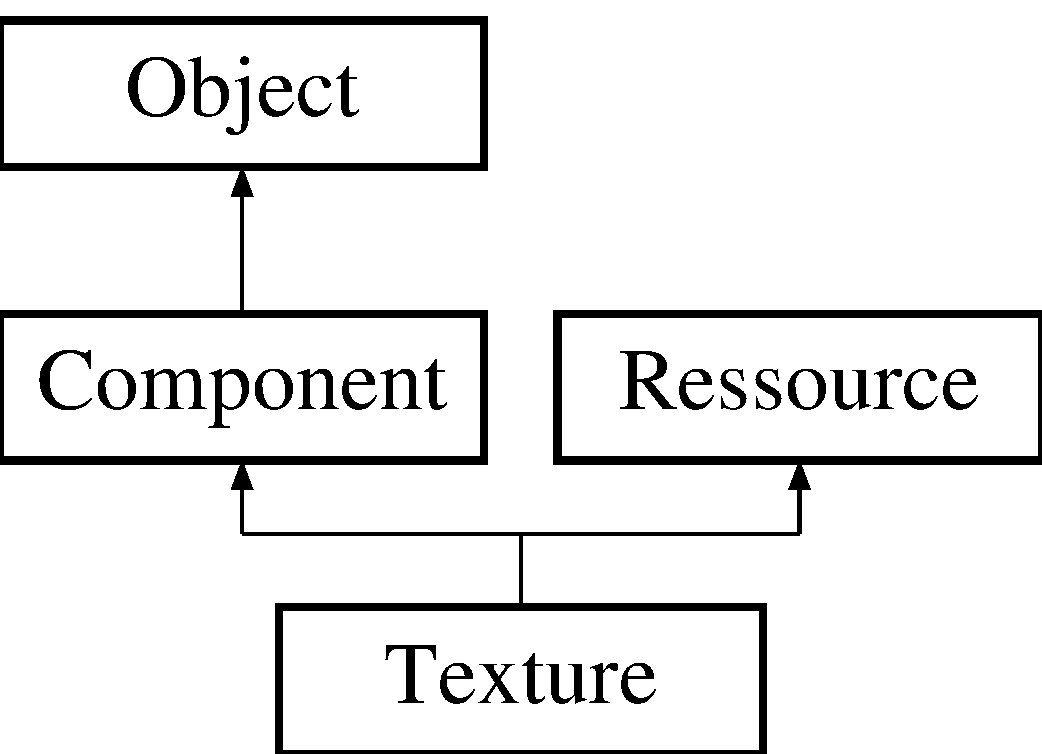
\includegraphics[height=3.000000cm]{class_texture}
\end{center}
\end{figure}
\subsection*{Public Member Functions}
\begin{DoxyCompactItemize}
\item 
\hypertarget{class_texture_ad90cdf5df00d3bd3e2f8585156b390eb}{
virtual const \hyperlink{class_r_t_t_i}{RTTI} \& {\bfseries getType} () const }
\label{class_texture_ad90cdf5df00d3bd3e2f8585156b390eb}

\item 
\hypertarget{class_texture_a25ab3a58fa60ccafe3e3883727bc63fc}{
{\bfseries Texture} (const std::string \&filePath)}
\label{class_texture_a25ab3a58fa60ccafe3e3883727bc63fc}

\item 
\hypertarget{class_texture_ab3fd325003ae75f683e86b511e5872a7}{
void {\bfseries bindTexture} () const }
\label{class_texture_ab3fd325003ae75f683e86b511e5872a7}

\item 
\hypertarget{class_texture_af4209ac00bda33ab1638dfd88e7951a0}{
GLuint {\bfseries getTexId} () const }
\label{class_texture_af4209ac00bda33ab1638dfd88e7951a0}

\item 
\hypertarget{class_texture_a249deb0d8e3d0e152cc50931b9145f81}{
Vec4f {\bfseries getPixel} (int u, int v) const }
\label{class_texture_a249deb0d8e3d0e152cc50931b9145f81}

\item 
\hypertarget{class_texture_a1f3e2bb88d139a8a15a11f88a34962fb}{
Vec4f {\bfseries getPixel} (float u, float v) const }
\label{class_texture_a1f3e2bb88d139a8a15a11f88a34962fb}

\item 
\hypertarget{class_texture_a496e7ecce88213f6190dcb65659ee9b4}{
int {\bfseries width} () const }
\label{class_texture_a496e7ecce88213f6190dcb65659ee9b4}

\item 
\hypertarget{class_texture_a0a5592fcf3a2270578880aed20c4bde0}{
int {\bfseries height} () const }
\label{class_texture_a0a5592fcf3a2270578880aed20c4bde0}

\end{DoxyCompactItemize}
\subsection*{Static Public Attributes}
\begin{DoxyCompactItemize}
\item 
\hypertarget{class_texture_a27590e7d9d79dd477e37fc0dacedf1f2}{
static const \hyperlink{class_r_t_t_i}{RTTI} {\bfseries TYPE}}
\label{class_texture_a27590e7d9d79dd477e37fc0dacedf1f2}

\end{DoxyCompactItemize}
\subsection*{Protected Member Functions}
\begin{DoxyCompactItemize}
\item 
\hypertarget{class_texture_a48e6b8ac86268c48111d7aee8a9ab93b}{
SDL\_\-Surface $\ast$ {\bfseries flipSurface} (SDL\_\-Surface $\ast$surface)}
\label{class_texture_a48e6b8ac86268c48111d7aee8a9ab93b}

\item 
\hypertarget{class_texture_a6b5ca734aab4547f7847ff2c8cc39f09}{
GLuint {\bfseries loadTexture} (const char $\ast$filename, bool useMipMap)}
\label{class_texture_a6b5ca734aab4547f7847ff2c8cc39f09}

\end{DoxyCompactItemize}
\subsection*{Protected Attributes}
\begin{DoxyCompactItemize}
\item 
\hypertarget{class_texture_a4b6c998e726cb9e63cdd3122d961290e}{
GLuint {\bfseries glTexObject}}
\label{class_texture_a4b6c998e726cb9e63cdd3122d961290e}

\item 
\hypertarget{class_texture_a3e8720fe713ee621f587d4bdbfcb8d12}{
std::string {\bfseries ressourceName}}
\label{class_texture_a3e8720fe713ee621f587d4bdbfcb8d12}

\item 
\hypertarget{class_texture_ad04401a2c4b6795ecdb0addd47a41651}{
SDL\_\-Surface $\ast$ {\bfseries textureMemory}}
\label{class_texture_ad04401a2c4b6795ecdb0addd47a41651}

\end{DoxyCompactItemize}
\subsection*{Friends}
\begin{DoxyCompactItemize}
\item 
\hypertarget{class_texture_ac98d07dd8f7b70e16ccb9a01abf56b9c}{
class {\bfseries boost::serialization::access}}
\label{class_texture_ac98d07dd8f7b70e16ccb9a01abf56b9c}

\end{DoxyCompactItemize}


The documentation for this class was generated from the following files:\begin{DoxyCompactItemize}
\item 
Texture.h\item 
Texture.cpp\end{DoxyCompactItemize}

\hypertarget{class_track_ball_camera}{
\section{TrackBallCamera Class Reference}
\label{class_track_ball_camera}\index{TrackBallCamera@{TrackBallCamera}}
}
\subsection*{Public Member Functions}
\begin{DoxyCompactItemize}
\item 
\hypertarget{class_track_ball_camera_adbd6e929a53521c1511379cee2efe5b2}{
{\bfseries TrackBallCamera} (\hyperlink{class_transform}{Transform} $\ast$trans)}
\label{class_track_ball_camera_adbd6e929a53521c1511379cee2efe5b2}

\item 
\hypertarget{class_track_ball_camera_a7a700f13749637899fb8749e8d136598}{
virtual void {\bfseries OnMouseMotion} (const SDL\_\-MouseMotionEvent \&event)}
\label{class_track_ball_camera_a7a700f13749637899fb8749e8d136598}

\item 
\hypertarget{class_track_ball_camera_a68e4695d4439a0f1a9dffdc474f9bcf2}{
virtual void {\bfseries OnMouseButton} (const SDL\_\-MouseButtonEvent \&event)}
\label{class_track_ball_camera_a68e4695d4439a0f1a9dffdc474f9bcf2}

\item 
\hypertarget{class_track_ball_camera_ac9d63bf5e2cc37176266d0f9002b6182}{
virtual void {\bfseries OnKeyboard} (const SDL\_\-KeyboardEvent \&event)}
\label{class_track_ball_camera_ac9d63bf5e2cc37176266d0f9002b6182}

\item 
\hypertarget{class_track_ball_camera_a592b46a7423b31dcdad6f6a7e6aff1a7}{
virtual void {\bfseries look} (float elapsed\_\-time)}
\label{class_track_ball_camera_a592b46a7423b31dcdad6f6a7e6aff1a7}

\item 
\hypertarget{class_track_ball_camera_a9942af262cd33039575f5c703304cc44}{
virtual void {\bfseries setMotionSensivity} (double sensivity)}
\label{class_track_ball_camera_a9942af262cd33039575f5c703304cc44}

\item 
\hypertarget{class_track_ball_camera_a55305b75b15ea49df24b89d591798661}{
virtual void {\bfseries setScrollSensivity} (double sensivity)}
\label{class_track_ball_camera_a55305b75b15ea49df24b89d591798661}

\end{DoxyCompactItemize}
\subsection*{Protected Attributes}
\begin{DoxyCompactItemize}
\item 
\hypertarget{class_track_ball_camera_af0d678af918c1887f5de5ae4b5e0960f}{
\hyperlink{class_transform}{Transform} $\ast$ {\bfseries transform}}
\label{class_track_ball_camera_af0d678af918c1887f5de5ae4b5e0960f}

\item 
\hypertarget{class_track_ball_camera_a097812817ed3ec665c76a38f71d8e133}{
double {\bfseries \_\-motionSensivity}}
\label{class_track_ball_camera_a097812817ed3ec665c76a38f71d8e133}

\item 
\hypertarget{class_track_ball_camera_ac24ec13cfb6134d7e064ba1052f08e23}{
double {\bfseries \_\-scrollSensivity}}
\label{class_track_ball_camera_ac24ec13cfb6134d7e064ba1052f08e23}

\item 
\hypertarget{class_track_ball_camera_a266fb5bce739065590ea94af85f6db96}{
bool {\bfseries \_\-hold}}
\label{class_track_ball_camera_a266fb5bce739065590ea94af85f6db96}

\item 
\hypertarget{class_track_ball_camera_aeceb35b6b038fa4f756e5098b37ef9f4}{
double {\bfseries \_\-distance}}
\label{class_track_ball_camera_aeceb35b6b038fa4f756e5098b37ef9f4}

\item 
\hypertarget{class_track_ball_camera_ad126b1c4d4e9e6bd8942015e7a19ebcc}{
double {\bfseries \_\-angleY}}
\label{class_track_ball_camera_ad126b1c4d4e9e6bd8942015e7a19ebcc}

\item 
\hypertarget{class_track_ball_camera_a785783601aa752acffad8c227a486271}{
double {\bfseries \_\-angleZ}}
\label{class_track_ball_camera_a785783601aa752acffad8c227a486271}

\item 
\hypertarget{class_track_ball_camera_ae9e9a83186de591c76ff43c7a1222d2b}{
SDL\_\-Cursor $\ast$ {\bfseries \_\-hand1}}
\label{class_track_ball_camera_ae9e9a83186de591c76ff43c7a1222d2b}

\item 
\hypertarget{class_track_ball_camera_a3cf8251a5a65b3cf5b93ddbf811d165c}{
SDL\_\-Cursor $\ast$ {\bfseries \_\-hand2}}
\label{class_track_ball_camera_a3cf8251a5a65b3cf5b93ddbf811d165c}

\end{DoxyCompactItemize}


The documentation for this class was generated from the following files:\begin{DoxyCompactItemize}
\item 
trackballcamera.h\item 
trackballcamera.cpp\end{DoxyCompactItemize}

\hypertarget{class_transform}{
\section{Transform Class Reference}
\label{class_transform}\index{Transform@{Transform}}
}
Inheritance diagram for Transform:\begin{figure}[H]
\begin{center}
\leavevmode
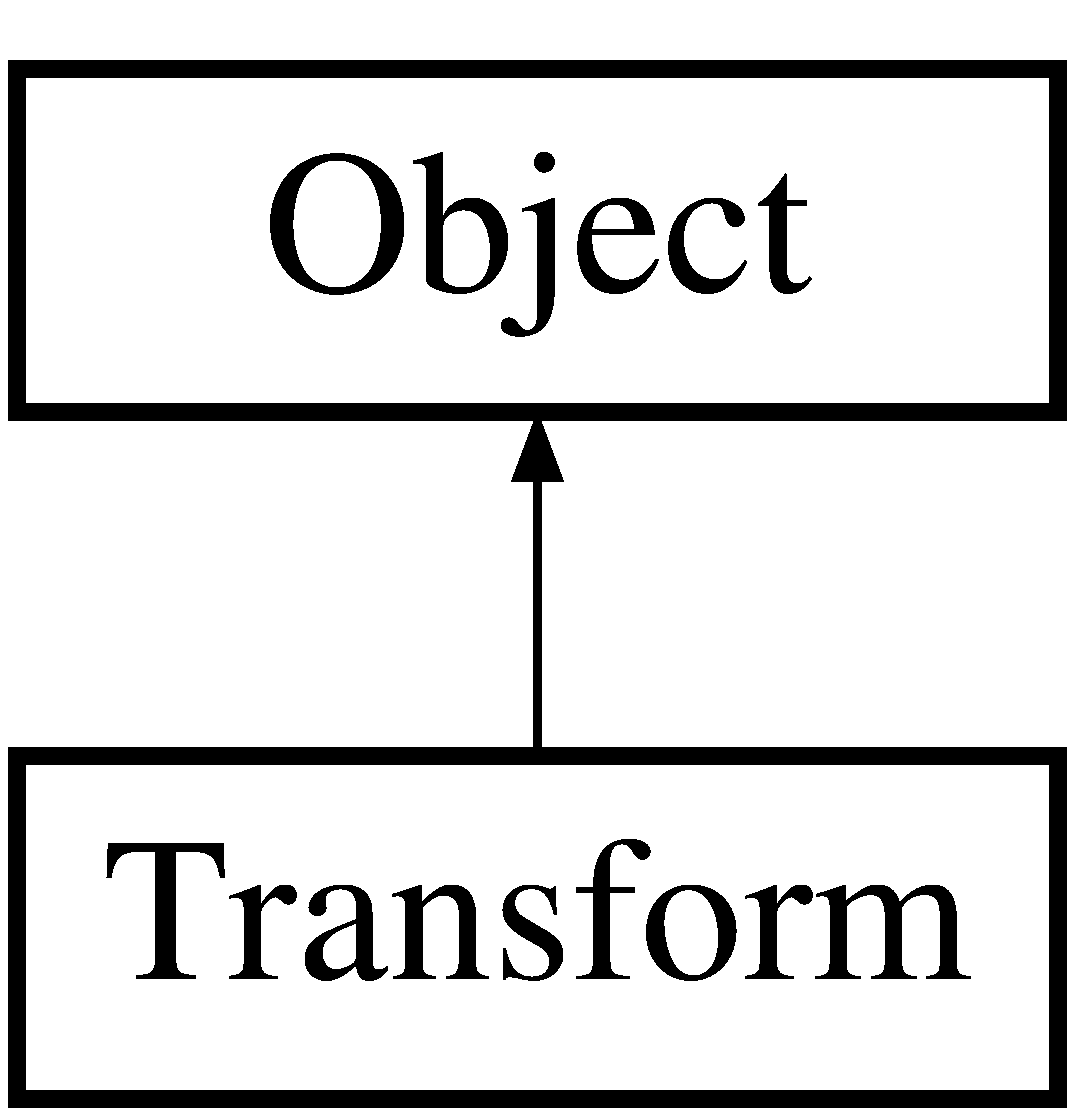
\includegraphics[height=2.000000cm]{class_transform}
\end{center}
\end{figure}
\subsection*{Public Types}
\begin{DoxyCompactItemize}
\item 
\hypertarget{class_transform_af3334261b0dc6bd65a7666bb5878db6c}{
typedef std::vector$<$ \hyperlink{class_transform}{Transform} $\ast$ $>$::const\_\-iterator {\bfseries ChildrenIterator}}
\label{class_transform_af3334261b0dc6bd65a7666bb5878db6c}

\end{DoxyCompactItemize}
\subsection*{Public Member Functions}
\begin{DoxyCompactItemize}
\item 
\hypertarget{class_transform_a8fd5df93229c1897055d7c9f0e5021ec}{
virtual const \hyperlink{class_r_t_t_i}{RTTI} \& {\bfseries getType} () const }
\label{class_transform_a8fd5df93229c1897055d7c9f0e5021ec}

\item 
\hypertarget{class_transform_a3f5a7ad019f402b52e5c7fed3699f01f}{
{\bfseries Transform} (Vec3f const \&pos)}
\label{class_transform_a3f5a7ad019f402b52e5c7fed3699f01f}

\item 
\hypertarget{class_transform_aa7a387108cf421888952b454d641895b}{
{\bfseries Transform} (const \hyperlink{class_transform}{Transform} \&transform)}
\label{class_transform_aa7a387108cf421888952b454d641895b}

\item 
\hypertarget{class_transform_a92d05e13bee5846f0895e097d55a0235}{
void {\bfseries setGameObject} (\hyperlink{class_game_object}{GameObject} $\ast$object)}
\label{class_transform_a92d05e13bee5846f0895e097d55a0235}

\item 
\hypertarget{class_transform_a64fefa4ce638359dffa28147d010c88c}{
\hyperlink{class_game_object}{GameObject} $\ast$ {\bfseries getGameObject} () const }
\label{class_transform_a64fefa4ce638359dffa28147d010c88c}

\item 
\hypertarget{class_transform_ad7d487d8508540f04b4caf3f9dd4dad2}{
void {\bfseries addChild} (\hyperlink{class_transform}{Transform} $\ast$child)}
\label{class_transform_ad7d487d8508540f04b4caf3f9dd4dad2}

\item 
\hypertarget{class_transform_a8c40957cdc496f51a993d252bc8fa459}{
void {\bfseries attachChild} (\hyperlink{class_transform}{Transform} $\ast$child)}
\label{class_transform_a8c40957cdc496f51a993d252bc8fa459}

\item 
\hypertarget{class_transform_a9d371d071641600820959f42670502ce}{
void {\bfseries removeChild} (\hyperlink{class_transform}{Transform} $\ast$child)}
\label{class_transform_a9d371d071641600820959f42670502ce}

\item 
\hypertarget{class_transform_add6687cbcdb5e3a586ee8470237f109b}{
void {\bfseries removeChild} (int index)}
\label{class_transform_add6687cbcdb5e3a586ee8470237f109b}

\item 
\hypertarget{class_transform_a7961b68e168fd48a7c6a0e7a378acfeb}{
ChildrenIterator {\bfseries getChildrenIteratorBegin} () const }
\label{class_transform_a7961b68e168fd48a7c6a0e7a378acfeb}

\item 
\hypertarget{class_transform_ad12f0221301787ba9b806e1398f56f9d}{
ChildrenIterator {\bfseries getChildrenIteratorEnd} () const }
\label{class_transform_ad12f0221301787ba9b806e1398f56f9d}

\item 
\hypertarget{class_transform_ae09f6770d60d2644d36eb666899a91ed}{
int {\bfseries getChildCount} () const }
\label{class_transform_ae09f6770d60d2644d36eb666899a91ed}

\item 
\hypertarget{class_transform_a79b644e5db68374184142d8d95df6934}{
\hyperlink{class_transform}{Transform} $\ast$ {\bfseries getChild} (int index)}
\label{class_transform_a79b644e5db68374184142d8d95df6934}

\item 
\hypertarget{class_transform_ad9f5a1d8320c3280bff5189b8e800b34}{
int {\bfseries getChildIndex} (\hyperlink{class_transform}{Transform} $\ast$child) const }
\label{class_transform_ad9f5a1d8320c3280bff5189b8e800b34}

\item 
\hypertarget{class_transform_ae3e8acbd25d7d171aff00da038f79a9a}{
\hyperlink{class_transform}{Transform} $\ast$ {\bfseries getParent} ()}
\label{class_transform_ae3e8acbd25d7d171aff00da038f79a9a}

\item 
\hypertarget{class_transform_a0bbb28cce7bca9363703b41ca10dcc57}{
void {\bfseries setParent} (\hyperlink{class_transform}{Transform} $\ast$par)}
\label{class_transform_a0bbb28cce7bca9363703b41ca10dcc57}

\item 
void \hyperlink{class_transform_a5a8d1890adf4dbba15a436f55f21c601}{setPosition} (const Vec3f \&pos)
\item 
void \hyperlink{class_transform_a08ced4e72301c25f99dedd54859fb23b}{setWorldPosition} (const Vec3f \&pos)
\item 
void \hyperlink{class_transform_a42d7de04d07befc5f7e5fd53c5ea7a46}{setScale} (const Vec3f \&scal)
\item 
void \hyperlink{class_transform_abe5b02d0f0bdcb854c26f1b81a4affde}{setWorldScale} (const Vec3f \&scal)
\item 
void \hyperlink{class_transform_a81bd0c59e3e584f6cefc63de81de7471}{setRotation} (const Vec3f \&rot)
\item 
\hypertarget{class_transform_a6fec9382d9851c08c303fbad1ae51f51}{
void {\bfseries translate} (float x, float y, float z)}
\label{class_transform_a6fec9382d9851c08c303fbad1ae51f51}

\item 
\hypertarget{class_transform_a707167a0cf2b279459b7b17a5e8270aa}{
void {\bfseries translate} (const Vec3f \&translation)}
\label{class_transform_a707167a0cf2b279459b7b17a5e8270aa}

\item 
\hypertarget{class_transform_a56f65b9bab2981aa800d3559823ad1b7}{
void {\bfseries scale} (float x, float y, float z)}
\label{class_transform_a56f65b9bab2981aa800d3559823ad1b7}

\item 
\hypertarget{class_transform_a1e0ef8fc5f8a4c84f0f4b13b39e250cc}{
void {\bfseries scale} (const Vec3f \&scaling)}
\label{class_transform_a1e0ef8fc5f8a4c84f0f4b13b39e250cc}

\item 
void \hyperlink{class_transform_a49da2af362feeaf653e09216d2e67314}{rotate} (float rx, float ry, float rz, SpaceOfReferenceEnum reference=PARENT)
\item 
void \hyperlink{class_transform_ae5b4cdd5d9cf3e8c3ef67907fd1663c2}{rotate} (const Vec3f \&euler\_\-angles, SpaceOfReferenceEnum reference=PARENT)
\item 
void \hyperlink{class_transform_ab8ab1268af903a4302825dc44f567446}{rotate} (const Vec3f \&axis, float angle)
\item 
void \hyperlink{class_transform_a559d420570aded5e0a5db372dfd7f4fa}{lookAt} (const Vec3f \&targetPoint)
\item 
\hypertarget{class_transform_abb87ba961251c18c7964cf9dd50923fa}{
Vec3f {\bfseries getPosition} () const }
\label{class_transform_abb87ba961251c18c7964cf9dd50923fa}

\item 
\hypertarget{class_transform_a7f91e85beafc56a5da3c53b31d7e5eb2}{
Vec3f {\bfseries getWorldPosition} () const }
\label{class_transform_a7f91e85beafc56a5da3c53b31d7e5eb2}

\item 
\hypertarget{class_transform_a35628a3c05902445ad155de45418e1cb}{
Vec3f {\bfseries getScale} () const }
\label{class_transform_a35628a3c05902445ad155de45418e1cb}

\item 
\hypertarget{class_transform_adfedc5e72afe00288d1bf84939e1f09b}{
Vec3f {\bfseries getWorldScale} () const }
\label{class_transform_adfedc5e72afe00288d1bf84939e1f09b}

\item 
\hypertarget{class_transform_ad941bc86b36ad61fad7dd24389e443f3}{
Vec3f {\bfseries getRotation} () const }
\label{class_transform_ad941bc86b36ad61fad7dd24389e443f3}

\item 
Vec3f \hyperlink{class_transform_a5072a5bbe7c6f2655b15b84576af9b43}{getForward} () const 
\item 
Vec3f \hyperlink{class_transform_ac0946577a65bd758b1ac8871fe626b84}{getUp} () const 
\item 
Vec3f \hyperlink{class_transform_a046298794a6ef7496718c1508b506b8e}{getRight} () const 
\item 
\hypertarget{class_transform_ab767ab8fcc2788303d6dbc998b28f944}{
Mat3x3f {\bfseries getRotationMatrix} () const }
\label{class_transform_ab767ab8fcc2788303d6dbc998b28f944}

\item 
\hypertarget{class_transform_aed6f35d7acd26be90473ed42f8c23a89}{
Mat3x3f {\bfseries getWorldRotationMatrix} () const }
\label{class_transform_aed6f35d7acd26be90473ed42f8c23a89}

\item 
\hypertarget{class_transform_a7c990738fbadb5ad1001be23626bb2c8}{
Mat4x4f {\bfseries getTransformMatrix} () const }
\label{class_transform_a7c990738fbadb5ad1001be23626bb2c8}

\item 
Mat4x4f \hyperlink{class_transform_acdd5b97256cce34a3581fe027b2a331f}{getInverseTransformMatrix} () const 
\item 
\hypertarget{class_transform_a36af2906e513a2a7f94a73e90fcd86d2}{
Mat4x4f {\bfseries getWorldTransformMatrix} () const }
\label{class_transform_a36af2906e513a2a7f94a73e90fcd86d2}

\item 
\hypertarget{class_transform_aad951114815c5309cc15466cd7446a36}{
Mat4x4f {\bfseries getWorldInverseTransformMatrix} () const }
\label{class_transform_aad951114815c5309cc15466cd7446a36}

\item 
\hypertarget{class_transform_a12a6ce5dea580d99c46911968471d283}{
Mat4x4f {\bfseries getWorldViewMatrix} () const }
\label{class_transform_a12a6ce5dea580d99c46911968471d283}

\item 
\hypertarget{class_transform_a403bb8391d10095c7ce5af0d3405358f}{
Mat4x4f {\bfseries getWorldInverseViewMatrix} () const }
\label{class_transform_a403bb8391d10095c7ce5af0d3405358f}

\item 
\hypertarget{class_transform_ad82fc7d715d43b2708eb1c78e2c59167}{
void {\bfseries applyTransform} () const }
\label{class_transform_ad82fc7d715d43b2708eb1c78e2c59167}

\item 
\hypertarget{class_transform_ab949ddd4287a01f3443dcffbb9eef7c7}{
void {\bfseries applyWorldTransform} () const }
\label{class_transform_ab949ddd4287a01f3443dcffbb9eef7c7}

\item 
\hypertarget{class_transform_a0db6a1afc8535b20c2fc4cbd5099764b}{
void {\bfseries applyViewTransform} () const }
\label{class_transform_a0db6a1afc8535b20c2fc4cbd5099764b}

\item 
\hypertarget{class_transform_a0161434d698b7017f9a3eb56ece7547e}{
void {\bfseries applyWorldViewTransform} () const }
\label{class_transform_a0161434d698b7017f9a3eb56ece7547e}

\item 
void \hyperlink{class_transform_a52689327a6d1fabd443da6191251e4b9}{\_\-updateWorldPosition} ()
\item 
void \hyperlink{class_transform_ae8bcdae14fdc45b5b1f1a54f55b82341}{\_\-updateTransformMatrix} ()
\item 
void \hyperlink{class_transform_a3d26f7bc1a10b83809f3780458f5361d}{\_\-updateWorldTransformMatrix} ()
\item 
void \hyperlink{class_transform_a627cc3ba8984b755b42ab629c7d027ea}{\_\-updateWorldRotationMatrix} ()
\end{DoxyCompactItemize}
\subsection*{Static Public Attributes}
\begin{DoxyCompactItemize}
\item 
\hypertarget{class_transform_a6c99a0f2b5cd6f81948b950c695f09a8}{
static const \hyperlink{class_r_t_t_i}{RTTI} {\bfseries TYPE}}
\label{class_transform_a6c99a0f2b5cd6f81948b950c695f09a8}

\end{DoxyCompactItemize}
\subsection*{Protected Attributes}
\begin{DoxyCompactItemize}
\item 
\hypertarget{class_transform_aeae6186d24a6968ab1cc423e6275edd0}{
\hyperlink{class_game_object}{GameObject} $\ast$ {\bfseries gameObject}}
\label{class_transform_aeae6186d24a6968ab1cc423e6275edd0}

\item 
\hypertarget{class_transform_aa1e92491c9905869a108ec09a08e5eb4}{
\hyperlink{class_transform}{Transform} $\ast$ {\bfseries parent}}
\label{class_transform_aa1e92491c9905869a108ec09a08e5eb4}

\item 
\hypertarget{class_transform_aba90cae9b61c6c614cd7b1a8151c24bd}{
std::vector$<$ \hyperlink{class_transform}{Transform} $\ast$ $>$ {\bfseries children}}
\label{class_transform_aba90cae9b61c6c614cd7b1a8151c24bd}

\item 
\hypertarget{class_transform_ade2b0121437dc8ffe92136d6d3592963}{
Vec3f {\bfseries position}}
\label{class_transform_ade2b0121437dc8ffe92136d6d3592963}

\item 
\hypertarget{class_transform_aefb83556a032d9ac4b76a9510461788a}{
Vec3f {\bfseries worldPosition}}
\label{class_transform_aefb83556a032d9ac4b76a9510461788a}

\item 
\hypertarget{class_transform_a06b04127dae94305ef74104aba545cbb}{
Vec3f {\bfseries scaling}}
\label{class_transform_a06b04127dae94305ef74104aba545cbb}

\item 
\hypertarget{class_transform_aa0fc7b67266edf8c8d7f62b534dee695}{
Vec3f {\bfseries worldScaling}}
\label{class_transform_aa0fc7b67266edf8c8d7f62b534dee695}

\item 
\hypertarget{class_transform_a6f903ef4b633f5efb267d422aa5c20fb}{
Vec3f {\bfseries eulerAngles}}
\label{class_transform_a6f903ef4b633f5efb267d422aa5c20fb}

\item 
\hypertarget{class_transform_ad18dc47412fadd14c60be416f030970c}{
Vec3f {\bfseries worldEulerAngles}}
\label{class_transform_ad18dc47412fadd14c60be416f030970c}

\item 
\hypertarget{class_transform_ad44aa94578d6f80d135b879add5eda1d}{
Mat3x3f {\bfseries rotationMatrix}}
\label{class_transform_ad44aa94578d6f80d135b879add5eda1d}

\item 
\hypertarget{class_transform_a0f8cf1d6d75de8543ab60feda8512f4f}{
Mat3x3f {\bfseries worldRotationMatrix}}
\label{class_transform_a0f8cf1d6d75de8543ab60feda8512f4f}

\item 
\hypertarget{class_transform_a2926f621763bb09c31e3507cc2446289}{
Mat4x4f {\bfseries transformMatrix}}
\label{class_transform_a2926f621763bb09c31e3507cc2446289}

\item 
\hypertarget{class_transform_a6d68c18e11ae927154ba5a539f1bf014}{
Mat4x4f {\bfseries worldTransformMatrix}}
\label{class_transform_a6d68c18e11ae927154ba5a539f1bf014}

\item 
\hypertarget{class_transform_a5df3356b2241cad2e6dec0ccf4baee44}{
bool {\bfseries \_\-hasMoved}}
\label{class_transform_a5df3356b2241cad2e6dec0ccf4baee44}

\end{DoxyCompactItemize}
\subsection*{Friends}
\begin{DoxyCompactItemize}
\item 
\hypertarget{class_transform_ac98d07dd8f7b70e16ccb9a01abf56b9c}{
class {\bfseries boost::serialization::access}}
\label{class_transform_ac98d07dd8f7b70e16ccb9a01abf56b9c}

\end{DoxyCompactItemize}


\subsection{Member Function Documentation}
\hypertarget{class_transform_ae8bcdae14fdc45b5b1f1a54f55b82341}{
\index{Transform@{Transform}!\_\-updateTransformMatrix@{\_\-updateTransformMatrix}}
\index{\_\-updateTransformMatrix@{\_\-updateTransformMatrix}!Transform@{Transform}}
\subsubsection[{\_\-updateTransformMatrix}]{\setlength{\rightskip}{0pt plus 5cm}void Transform::\_\-updateTransformMatrix (
\begin{DoxyParamCaption}
{}
\end{DoxyParamCaption}
)}}
\label{class_transform_ae8bcdae14fdc45b5b1f1a54f55b82341}
Called internally, updates and caches the local transform matrix from position rotation and scaling, calls \hyperlink{class_transform_a52689327a6d1fabd443da6191251e4b9}{\_\-updateWorldPosition()} \hypertarget{class_transform_a52689327a6d1fabd443da6191251e4b9}{
\index{Transform@{Transform}!\_\-updateWorldPosition@{\_\-updateWorldPosition}}
\index{\_\-updateWorldPosition@{\_\-updateWorldPosition}!Transform@{Transform}}
\subsubsection[{\_\-updateWorldPosition}]{\setlength{\rightskip}{0pt plus 5cm}void Transform::\_\-updateWorldPosition (
\begin{DoxyParamCaption}
{}
\end{DoxyParamCaption}
)}}
\label{class_transform_a52689327a6d1fabd443da6191251e4b9}
Called internally, updates and caches the world position given the one of the parent, propagates to childrens \hypertarget{class_transform_a627cc3ba8984b755b42ab629c7d027ea}{
\index{Transform@{Transform}!\_\-updateWorldRotationMatrix@{\_\-updateWorldRotationMatrix}}
\index{\_\-updateWorldRotationMatrix@{\_\-updateWorldRotationMatrix}!Transform@{Transform}}
\subsubsection[{\_\-updateWorldRotationMatrix}]{\setlength{\rightskip}{0pt plus 5cm}void Transform::\_\-updateWorldRotationMatrix (
\begin{DoxyParamCaption}
{}
\end{DoxyParamCaption}
)}}
\label{class_transform_a627cc3ba8984b755b42ab629c7d027ea}
Called internally, updates and caches the worl rotation matrix (R) from the parent, propagates to childrens \hypertarget{class_transform_a3d26f7bc1a10b83809f3780458f5361d}{
\index{Transform@{Transform}!\_\-updateWorldTransformMatrix@{\_\-updateWorldTransformMatrix}}
\index{\_\-updateWorldTransformMatrix@{\_\-updateWorldTransformMatrix}!Transform@{Transform}}
\subsubsection[{\_\-updateWorldTransformMatrix}]{\setlength{\rightskip}{0pt plus 5cm}void Transform::\_\-updateWorldTransformMatrix (
\begin{DoxyParamCaption}
{}
\end{DoxyParamCaption}
)}}
\label{class_transform_a3d26f7bc1a10b83809f3780458f5361d}
Called internally, updates and caches the worl transform (SRT) matrix from the parent, propagates to childrens \hypertarget{class_transform_a5072a5bbe7c6f2655b15b84576af9b43}{
\index{Transform@{Transform}!getForward@{getForward}}
\index{getForward@{getForward}!Transform@{Transform}}
\subsubsection[{getForward}]{\setlength{\rightskip}{0pt plus 5cm}Vec3f Transform::getForward (
\begin{DoxyParamCaption}
{}
\end{DoxyParamCaption}
) const}}
\label{class_transform_a5072a5bbe7c6f2655b15b84576af9b43}
Returns the forward vector of the frame in world space \hypertarget{class_transform_acdd5b97256cce34a3581fe027b2a331f}{
\index{Transform@{Transform}!getInverseTransformMatrix@{getInverseTransformMatrix}}
\index{getInverseTransformMatrix@{getInverseTransformMatrix}!Transform@{Transform}}
\subsubsection[{getInverseTransformMatrix}]{\setlength{\rightskip}{0pt plus 5cm}Mat4x4f Transform::getInverseTransformMatrix (
\begin{DoxyParamCaption}
{}
\end{DoxyParamCaption}
) const}}
\label{class_transform_acdd5b97256cce34a3581fe027b2a331f}
Returns the inverse of the transform matrix (used?) not taking into account the scaling \hypertarget{class_transform_a046298794a6ef7496718c1508b506b8e}{
\index{Transform@{Transform}!getRight@{getRight}}
\index{getRight@{getRight}!Transform@{Transform}}
\subsubsection[{getRight}]{\setlength{\rightskip}{0pt plus 5cm}Vec3f Transform::getRight (
\begin{DoxyParamCaption}
{}
\end{DoxyParamCaption}
) const}}
\label{class_transform_a046298794a6ef7496718c1508b506b8e}
Returns the right vector of the frame in world space \hypertarget{class_transform_ac0946577a65bd758b1ac8871fe626b84}{
\index{Transform@{Transform}!getUp@{getUp}}
\index{getUp@{getUp}!Transform@{Transform}}
\subsubsection[{getUp}]{\setlength{\rightskip}{0pt plus 5cm}Vec3f Transform::getUp (
\begin{DoxyParamCaption}
{}
\end{DoxyParamCaption}
) const}}
\label{class_transform_ac0946577a65bd758b1ac8871fe626b84}
Returns the up vector of the frame in world space \hypertarget{class_transform_a559d420570aded5e0a5db372dfd7f4fa}{
\index{Transform@{Transform}!lookAt@{lookAt}}
\index{lookAt@{lookAt}!Transform@{Transform}}
\subsubsection[{lookAt}]{\setlength{\rightskip}{0pt plus 5cm}void Transform::lookAt (
\begin{DoxyParamCaption}
\item[{const Vec3f \&}]{ targetPoint}
\end{DoxyParamCaption}
)}}
\label{class_transform_a559d420570aded5e0a5db372dfd7f4fa}
Sets the orientation of the transform so that it points to targetPoint with up vector being z world \hypertarget{class_transform_a49da2af362feeaf653e09216d2e67314}{
\index{Transform@{Transform}!rotate@{rotate}}
\index{rotate@{rotate}!Transform@{Transform}}
\subsubsection[{rotate}]{\setlength{\rightskip}{0pt plus 5cm}void Transform::rotate (
\begin{DoxyParamCaption}
\item[{float}]{ rx, }
\item[{float}]{ ry, }
\item[{float}]{ rz, }
\item[{SpaceOfReferenceEnum}]{ reference = {\ttfamily PARENT}}
\end{DoxyParamCaption}
)}}
\label{class_transform_a49da2af362feeaf653e09216d2e67314}
set the rotation of the transform, bad interface since rot are done xyz \hypertarget{class_transform_ae5b4cdd5d9cf3e8c3ef67907fd1663c2}{
\index{Transform@{Transform}!rotate@{rotate}}
\index{rotate@{rotate}!Transform@{Transform}}
\subsubsection[{rotate}]{\setlength{\rightskip}{0pt plus 5cm}void Transform::rotate (
\begin{DoxyParamCaption}
\item[{const Vec3f \&}]{ euler\_\-angles, }
\item[{SpaceOfReferenceEnum}]{ reference = {\ttfamily PARENT}}
\end{DoxyParamCaption}
)}}
\label{class_transform_ae5b4cdd5d9cf3e8c3ef67907fd1663c2}
set the rotation of the transform, bad interface since rot are done xyz \hypertarget{class_transform_ab8ab1268af903a4302825dc44f567446}{
\index{Transform@{Transform}!rotate@{rotate}}
\index{rotate@{rotate}!Transform@{Transform}}
\subsubsection[{rotate}]{\setlength{\rightskip}{0pt plus 5cm}void Transform::rotate (
\begin{DoxyParamCaption}
\item[{const Vec3f \&}]{ axis, }
\item[{float}]{ angle}
\end{DoxyParamCaption}
)}}
\label{class_transform_ab8ab1268af903a4302825dc44f567446}
Rotates the transform around an arbitrary axe in world space \hypertarget{class_transform_a5a8d1890adf4dbba15a436f55f21c601}{
\index{Transform@{Transform}!setPosition@{setPosition}}
\index{setPosition@{setPosition}!Transform@{Transform}}
\subsubsection[{setPosition}]{\setlength{\rightskip}{0pt plus 5cm}void Transform::setPosition (
\begin{DoxyParamCaption}
\item[{const Vec3f \&}]{ pos}
\end{DoxyParamCaption}
)}}
\label{class_transform_a5a8d1890adf4dbba15a436f55f21c601}
Unused, unmaintained \hypertarget{class_transform_a81bd0c59e3e584f6cefc63de81de7471}{
\index{Transform@{Transform}!setRotation@{setRotation}}
\index{setRotation@{setRotation}!Transform@{Transform}}
\subsubsection[{setRotation}]{\setlength{\rightskip}{0pt plus 5cm}void Transform::setRotation (
\begin{DoxyParamCaption}
\item[{const Vec3f \&}]{ rot}
\end{DoxyParamCaption}
)}}
\label{class_transform_a81bd0c59e3e584f6cefc63de81de7471}
Unused, unmaintained \hypertarget{class_transform_a42d7de04d07befc5f7e5fd53c5ea7a46}{
\index{Transform@{Transform}!setScale@{setScale}}
\index{setScale@{setScale}!Transform@{Transform}}
\subsubsection[{setScale}]{\setlength{\rightskip}{0pt plus 5cm}void Transform::setScale (
\begin{DoxyParamCaption}
\item[{const Vec3f \&}]{ scal}
\end{DoxyParamCaption}
)}}
\label{class_transform_a42d7de04d07befc5f7e5fd53c5ea7a46}
Unused, unmaintained \hypertarget{class_transform_a08ced4e72301c25f99dedd54859fb23b}{
\index{Transform@{Transform}!setWorldPosition@{setWorldPosition}}
\index{setWorldPosition@{setWorldPosition}!Transform@{Transform}}
\subsubsection[{setWorldPosition}]{\setlength{\rightskip}{0pt plus 5cm}void Transform::setWorldPosition (
\begin{DoxyParamCaption}
\item[{const Vec3f \&}]{ pos}
\end{DoxyParamCaption}
)}}
\label{class_transform_a08ced4e72301c25f99dedd54859fb23b}
Unused, unimplemented \hypertarget{class_transform_abe5b02d0f0bdcb854c26f1b81a4affde}{
\index{Transform@{Transform}!setWorldScale@{setWorldScale}}
\index{setWorldScale@{setWorldScale}!Transform@{Transform}}
\subsubsection[{setWorldScale}]{\setlength{\rightskip}{0pt plus 5cm}void Transform::setWorldScale (
\begin{DoxyParamCaption}
\item[{const Vec3f \&}]{ scal}
\end{DoxyParamCaption}
)}}
\label{class_transform_abe5b02d0f0bdcb854c26f1b81a4affde}
Unused, unimplemented 

The documentation for this class was generated from the following files:\begin{DoxyCompactItemize}
\item 
Transform.h\item 
Transform.cpp\end{DoxyCompactItemize}

\input{class_t_r_engine}
\input{class_t_r3_d_1_1_tri_mesh}
\input{struct_vertex}
\printindex
\end{document}
